\section{Performance Evaluation}
\label{sec:results}

This section describes the experimental evaluation of the proposed multi-tier video delivery architecture, including initial evaluation scenarios, metrics, methodology, and outcomes.
 
%\subsection{Methodology}
%
%We present three approaches to address the methodological problems identified in a edge/cloud multi-tier network for watching a video streaming: cloud-only 

\subsection{Experimental Setup}

%[29] Christian Kreuzberger, Daniel Posch, and Hermann Hellwagner. Amust framework - adaptive multimedia streaming simulation framework for ns-3 and ndnsim, 2016.
%[30] C. Mueller, S. Lederer, J. Poecher, and C. Timmerer. Demo paper: Libdash - an open source software library for the mpeg-dash standard. In 2013 IEEE International Conference on Multimedia and Expo Workshops (ICMEW), pages 1–2, July 2013.
% Per-title encode optimization, 2015. ; accessed 20-novembro-2019.

We use Adaptive Multimedia Streaming~(AMuSt)~\cite{kreuzberger2016amust} to implement a video streaming server, and the server is implemented through Dynamic Adaptive Streaming over HTTP~(DASH), with users that allow adaptive video streaming. The AMuSt framework provides a set of applications for producing and consuming adaptable videos based on the DASH standard. DASH functionality is provided by the libdash library~\cite{mueller2013ICMEW}, an open source library that provides an interface to the DASH standard. Currently, libdash is the official reference software for the DASH standard. We consider that users are interested in an available video with ten different bit rate representations \{235kbps, 375kbps, 560kbps, 560kbps, 750kbps, 1050kbps, 1750kbps, 2350kbps, 3000kbps, 4300kbps, 5800kbps\}, which are used by Netflix subsets~\cite{netflix:representation}. Each representation is divided into 2-second segments. All the experiments are executed once with a video of 1600 seconds~(800 segments). 
For simplicity, the multimedia content used in the simulation is deployed beforehand in the edge peering nodes. 

%Figure 3 shows the topology with three levels used in the experiments, each level \{1, 2 and 3\} is represented as a scenario.

%Dash server and the clients allowed to request a multimedia content in DASH format, was used the Adaptive Multimedia Streaming~(AMuSt). The AMust system allows a set o apps to produce and consume the adaptive video-based on Dash pattern. The DASH functionality is provided by the libdash library, an open source library that provides an interface to the DASH standard. Currently, libdash is the reference software official DASH standard.

We simulate the scenario in a binary tree topology with seven nodes and a Cloud Provider connected to the root node. The last four nodes are Access Points~(AP), and the others are edge peering points. Figure~\ref{fig:exp-setup-scenario} illustrates this scenario.

The AP nodes are implemented on wireless devices that communicate via IEEE 802.11g in 2.4GHz. The APs have wired connections to the edge peering points, while the end-users are wireless. Each user connected to the AP is located precisely 8 meters away from the AP. The Bandwidth available in each link can be seen in Figure~\ref{fig:exp-setup-scenario}.

We present three approaches to address the impacts identified in Section~\ref{sec:system-archi} into the edge/cloud multi-tier network, namely \textit{cloud-only}, \textit{edge cache}, and mobile-based scenarios. The cloud-only scenario uses only the Cloud Provider node to deliver the video content. On the other hand, the \textit{edge cache} approach uses nodes $1$ and $2$ as auxiliary nodes to deliver the video. The simulation starts with the users requesting the video from the cloud. When a congested link is detected, the edge cache below the link is turned on. Thereafter, the users receiving the video over the congested link are redirected to the edge nodes 1 and 2. 

The number of end-user devices communicating through each wireless AP may change over time due to the mobility of the end-user devices. In practice, the number of end-user devices connecting to the wireless AP changes frequently. 
To show the problems that can arise in such dynamic load scenarios, a connection change between the APs occurs. We then reran the second experiment, maintaining connections between users and edge nodes 1 and 2, but changing the connection between users and APs, emulating users' mobility. In this mobility scenario, half the users of each $AP_{i}$ go directly to $AP_{i + 2}$.
%Onde os metade dos usuários de cada $AP_{i}$ vão diretamente para o $AP_{i+2}$.
%Para mostrar os problemas que podem aparecer em tais cenários, e ocorre uma mudança de conexão entre os APs. Nós executamos novamente o segundo experimento mantendo as conexões entre os usuários e edge nodes, mas mudamos a conexão entre os usuários e os APs. 


\begin{figure}
    \centering
    %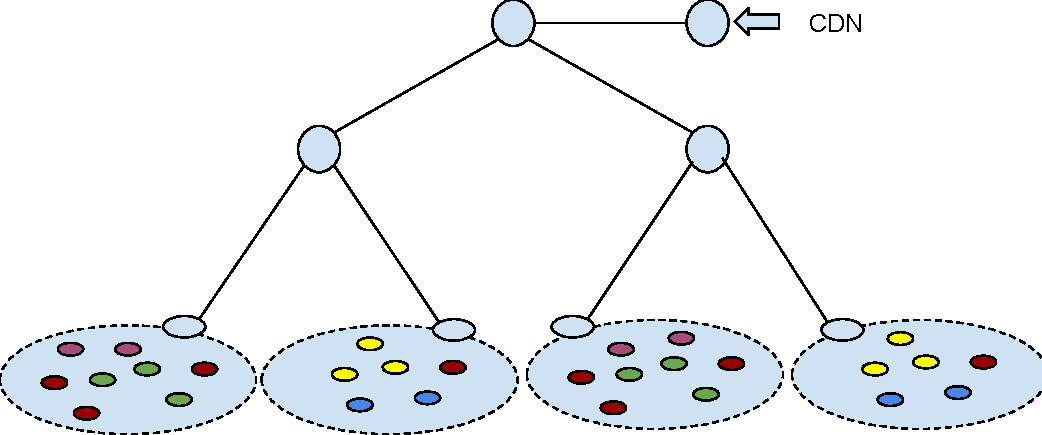
\includegraphics[width=0.9\linewidth]{images/exp-setup-scenario.pdf}
    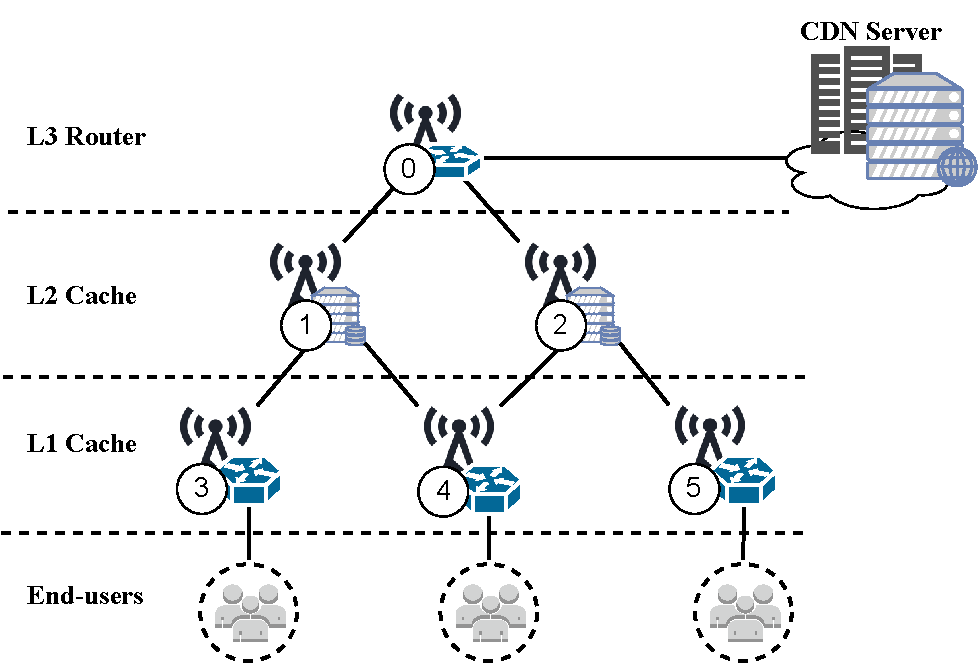
\includegraphics[width=\linewidth]{images/qoe-multi-level-2.pdf}
    \caption{A General Overview of the multi-tier network environment.}
    \label{fig:exp-setup-scenario}
\end{figure}

%To illustrate the idea, we assume tree topology. According to the guideline, a mobile backhaul network is modeled as a two-level hierarchical network. Wireless base stations are connected to aggregation nodes, e.g., service/packet data network gateway (S/P-GW) nodes. Furthermore, aggregation nodes are connected to core nodes, e.g., central office nodes. To the best of our knowledge, separation of traffic from one wireless base stations to multiple aggregation nodes, and from one aggregation node to multiple core nodes is not dominant in current mobile backhaul networks. Thus, we assume a tree-topology backhaul network


\subsection{QoE Assessment}

There are many QoE models in the literature. We describe how QoE metrics can be used to score user satisfaction. Firstly, each video quality chunk is computed by a logarithmic law over bitrates~\cite{Zhang:TransM13}, where a video quality model for DASH is proposed as shown in Equation~\ref{eq:equation-1}. Each video has $N$ segments and is encoded with $L$ bitrate levels. $r_i$ represents a specific bitrate level. At each step $i$, the quality of segment $i$, which is encoded at $l_i$ is defined as:

\begin{equation}\label{eq:equation-1}
q(r_i) = a_1 * log(a_2 * (r_i/ r_{|L|}))
\end{equation}
\vspace{0.05cm}

It is required a flexible QoE model that includes the most influential metrics to quantify long-term users' QoE. 
We consider Equation~\ref{eq:qoe-equation} from~\cite{bentaleb:2018:MSys}, which consists of four metrics: (a) the average chunk perceptual quality, (b) the average number of quality oscillations, (c) the average number of stall events and their durations, and (d) the startup delay. $K$ represents the total segments of the video, $S_{i}$ is the stall duration, and $ST_{i}$ is the startup delay of user $i$.

\begin{equation}\label{eq:qoe-equation}
\begin{split}
QoE_i = \frac{1}{K} \sum_{k=1}^{K}q(r_{k}) - \frac{1}{K-1} \sum_{k=1}^{K-1}|q(r_{k+1}) - q(r_{k})| \\
- \frac{1}{K}\sum_{k=1}^{K} S_{k} - ST_{i}
\end{split}
\end{equation}
\vspace{0.05cm}

The $QoE_{i}$ for each user $i$ can range from 1 to 5, where 1 = bad, 2 = poor, 3 = fair, 4 = good, and 5 = excellent.

%
% \begin{figure*}
%     \centering
%     \subfigure[]{
%     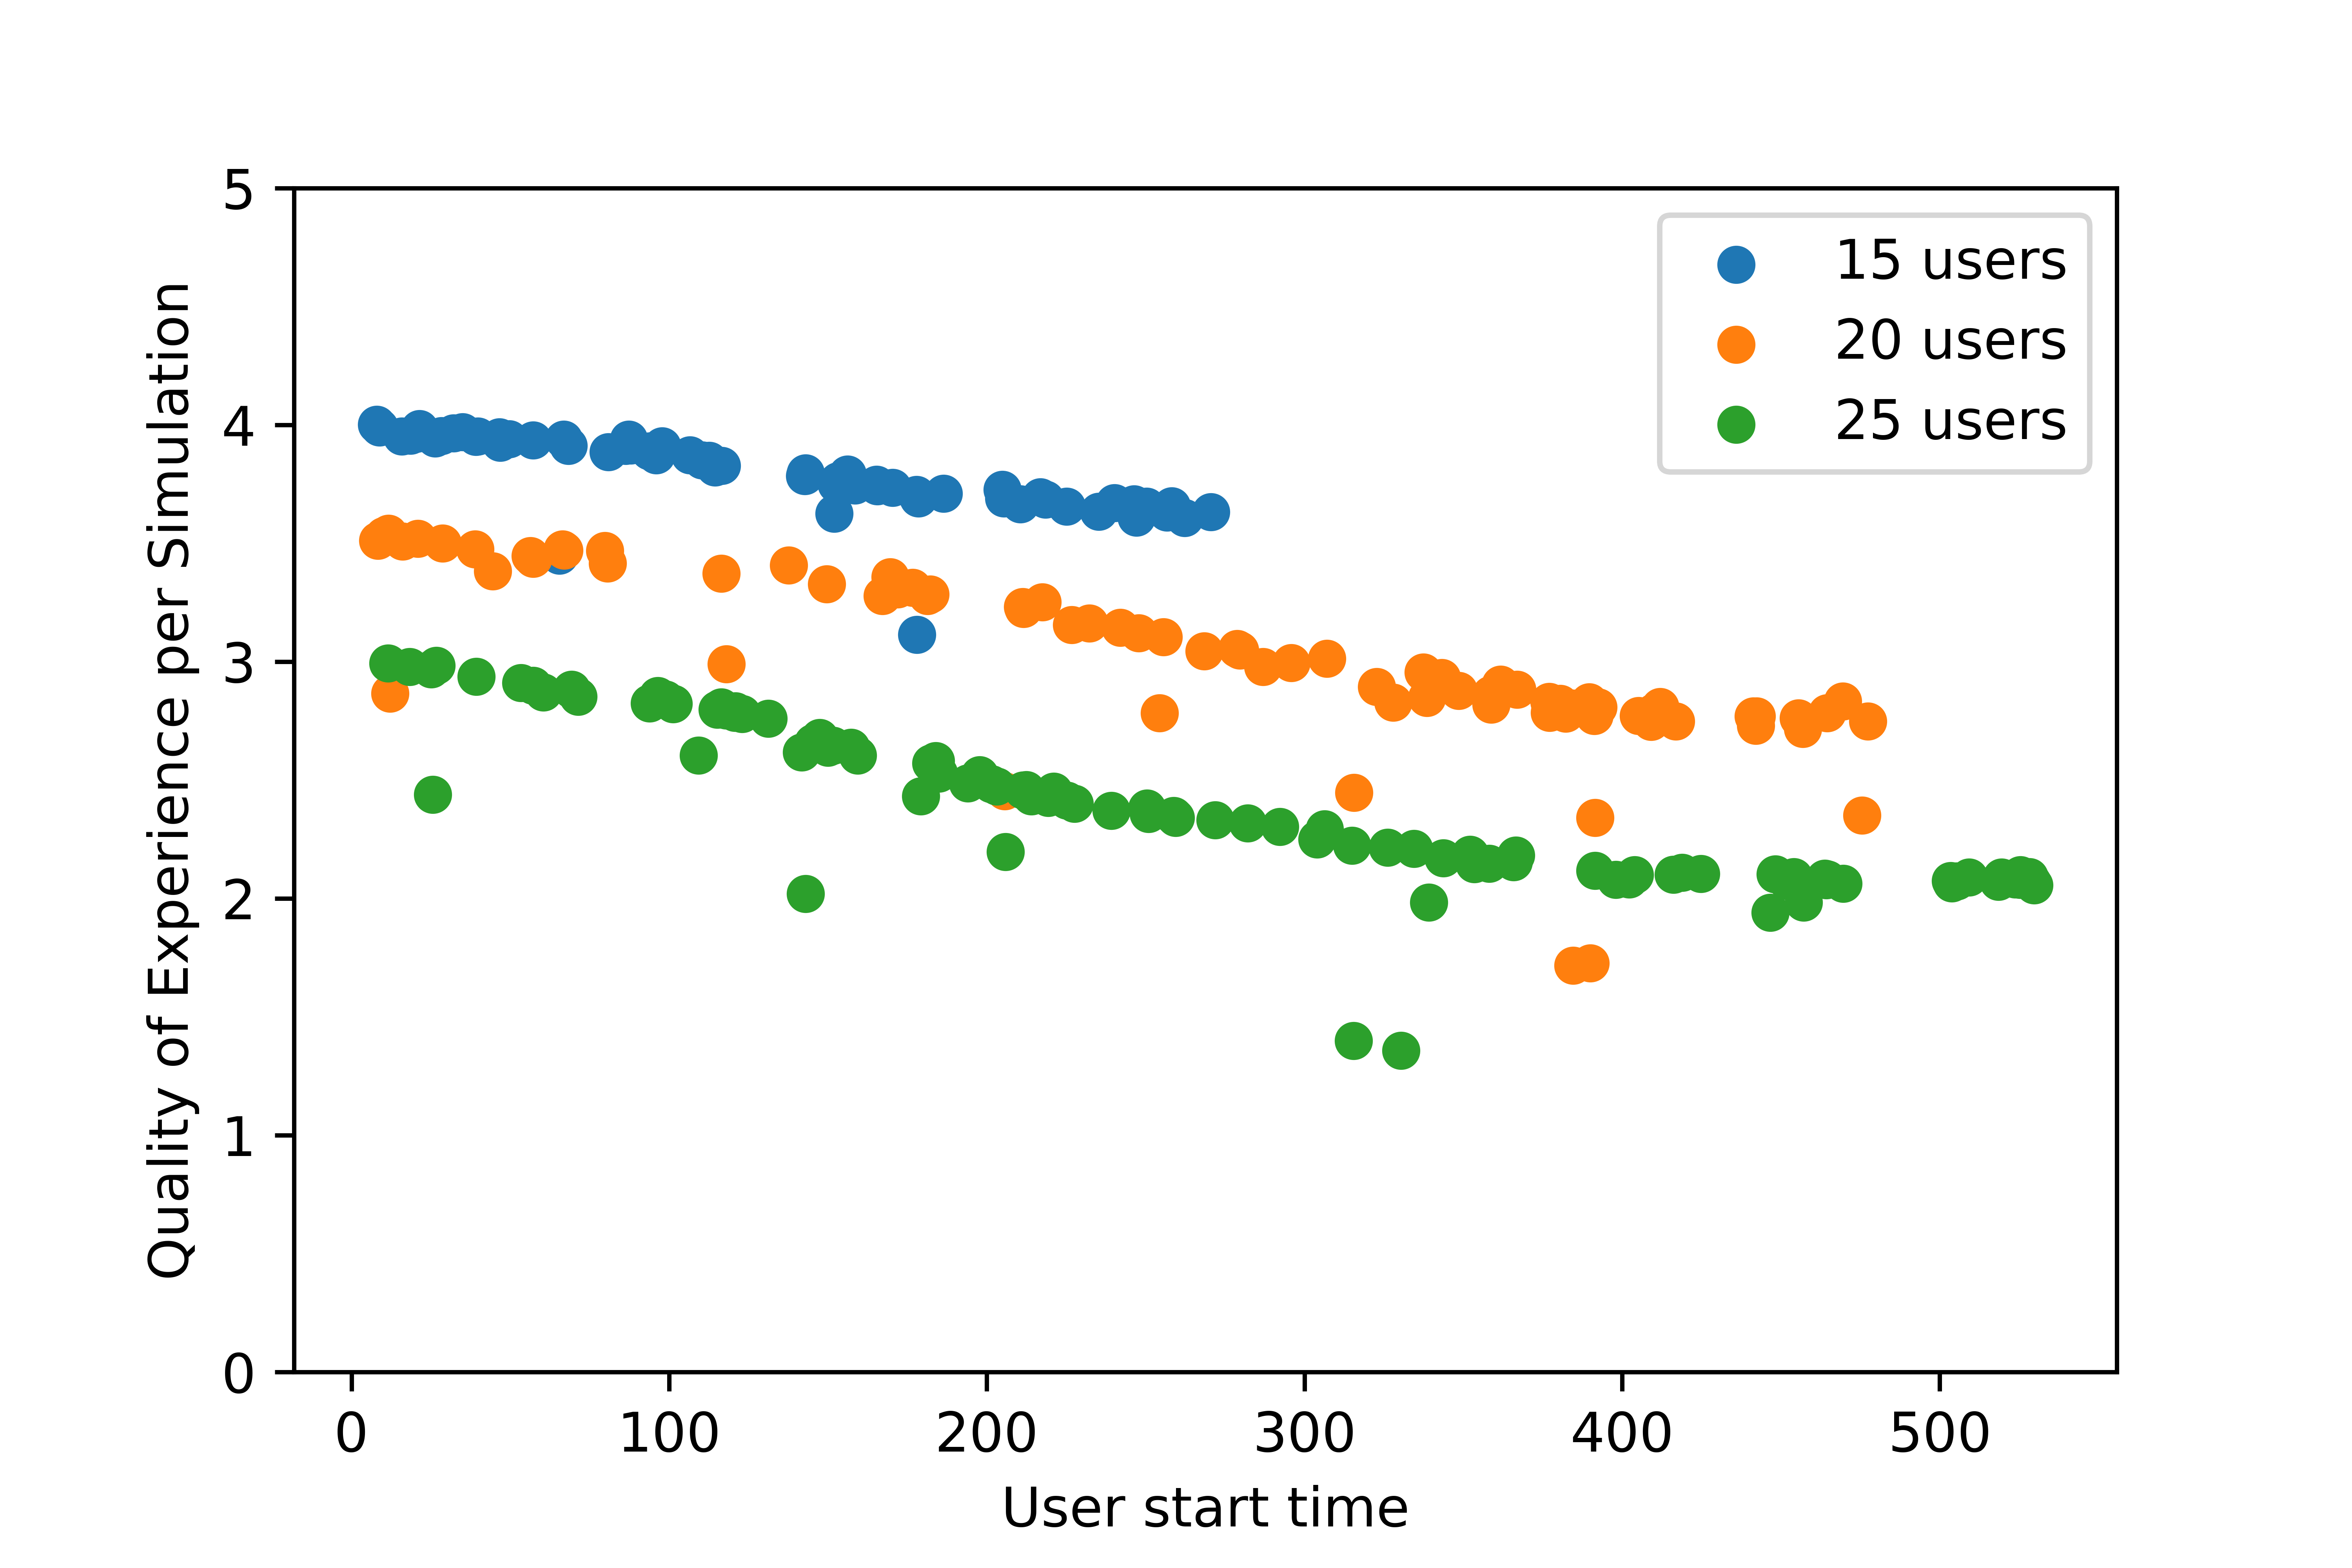
\includegraphics[width=0.45\linewidth]{images/QoECompare.png}
%     \label{fig:red-comparison-plot}
%     }
%     \subfigure[]{
%     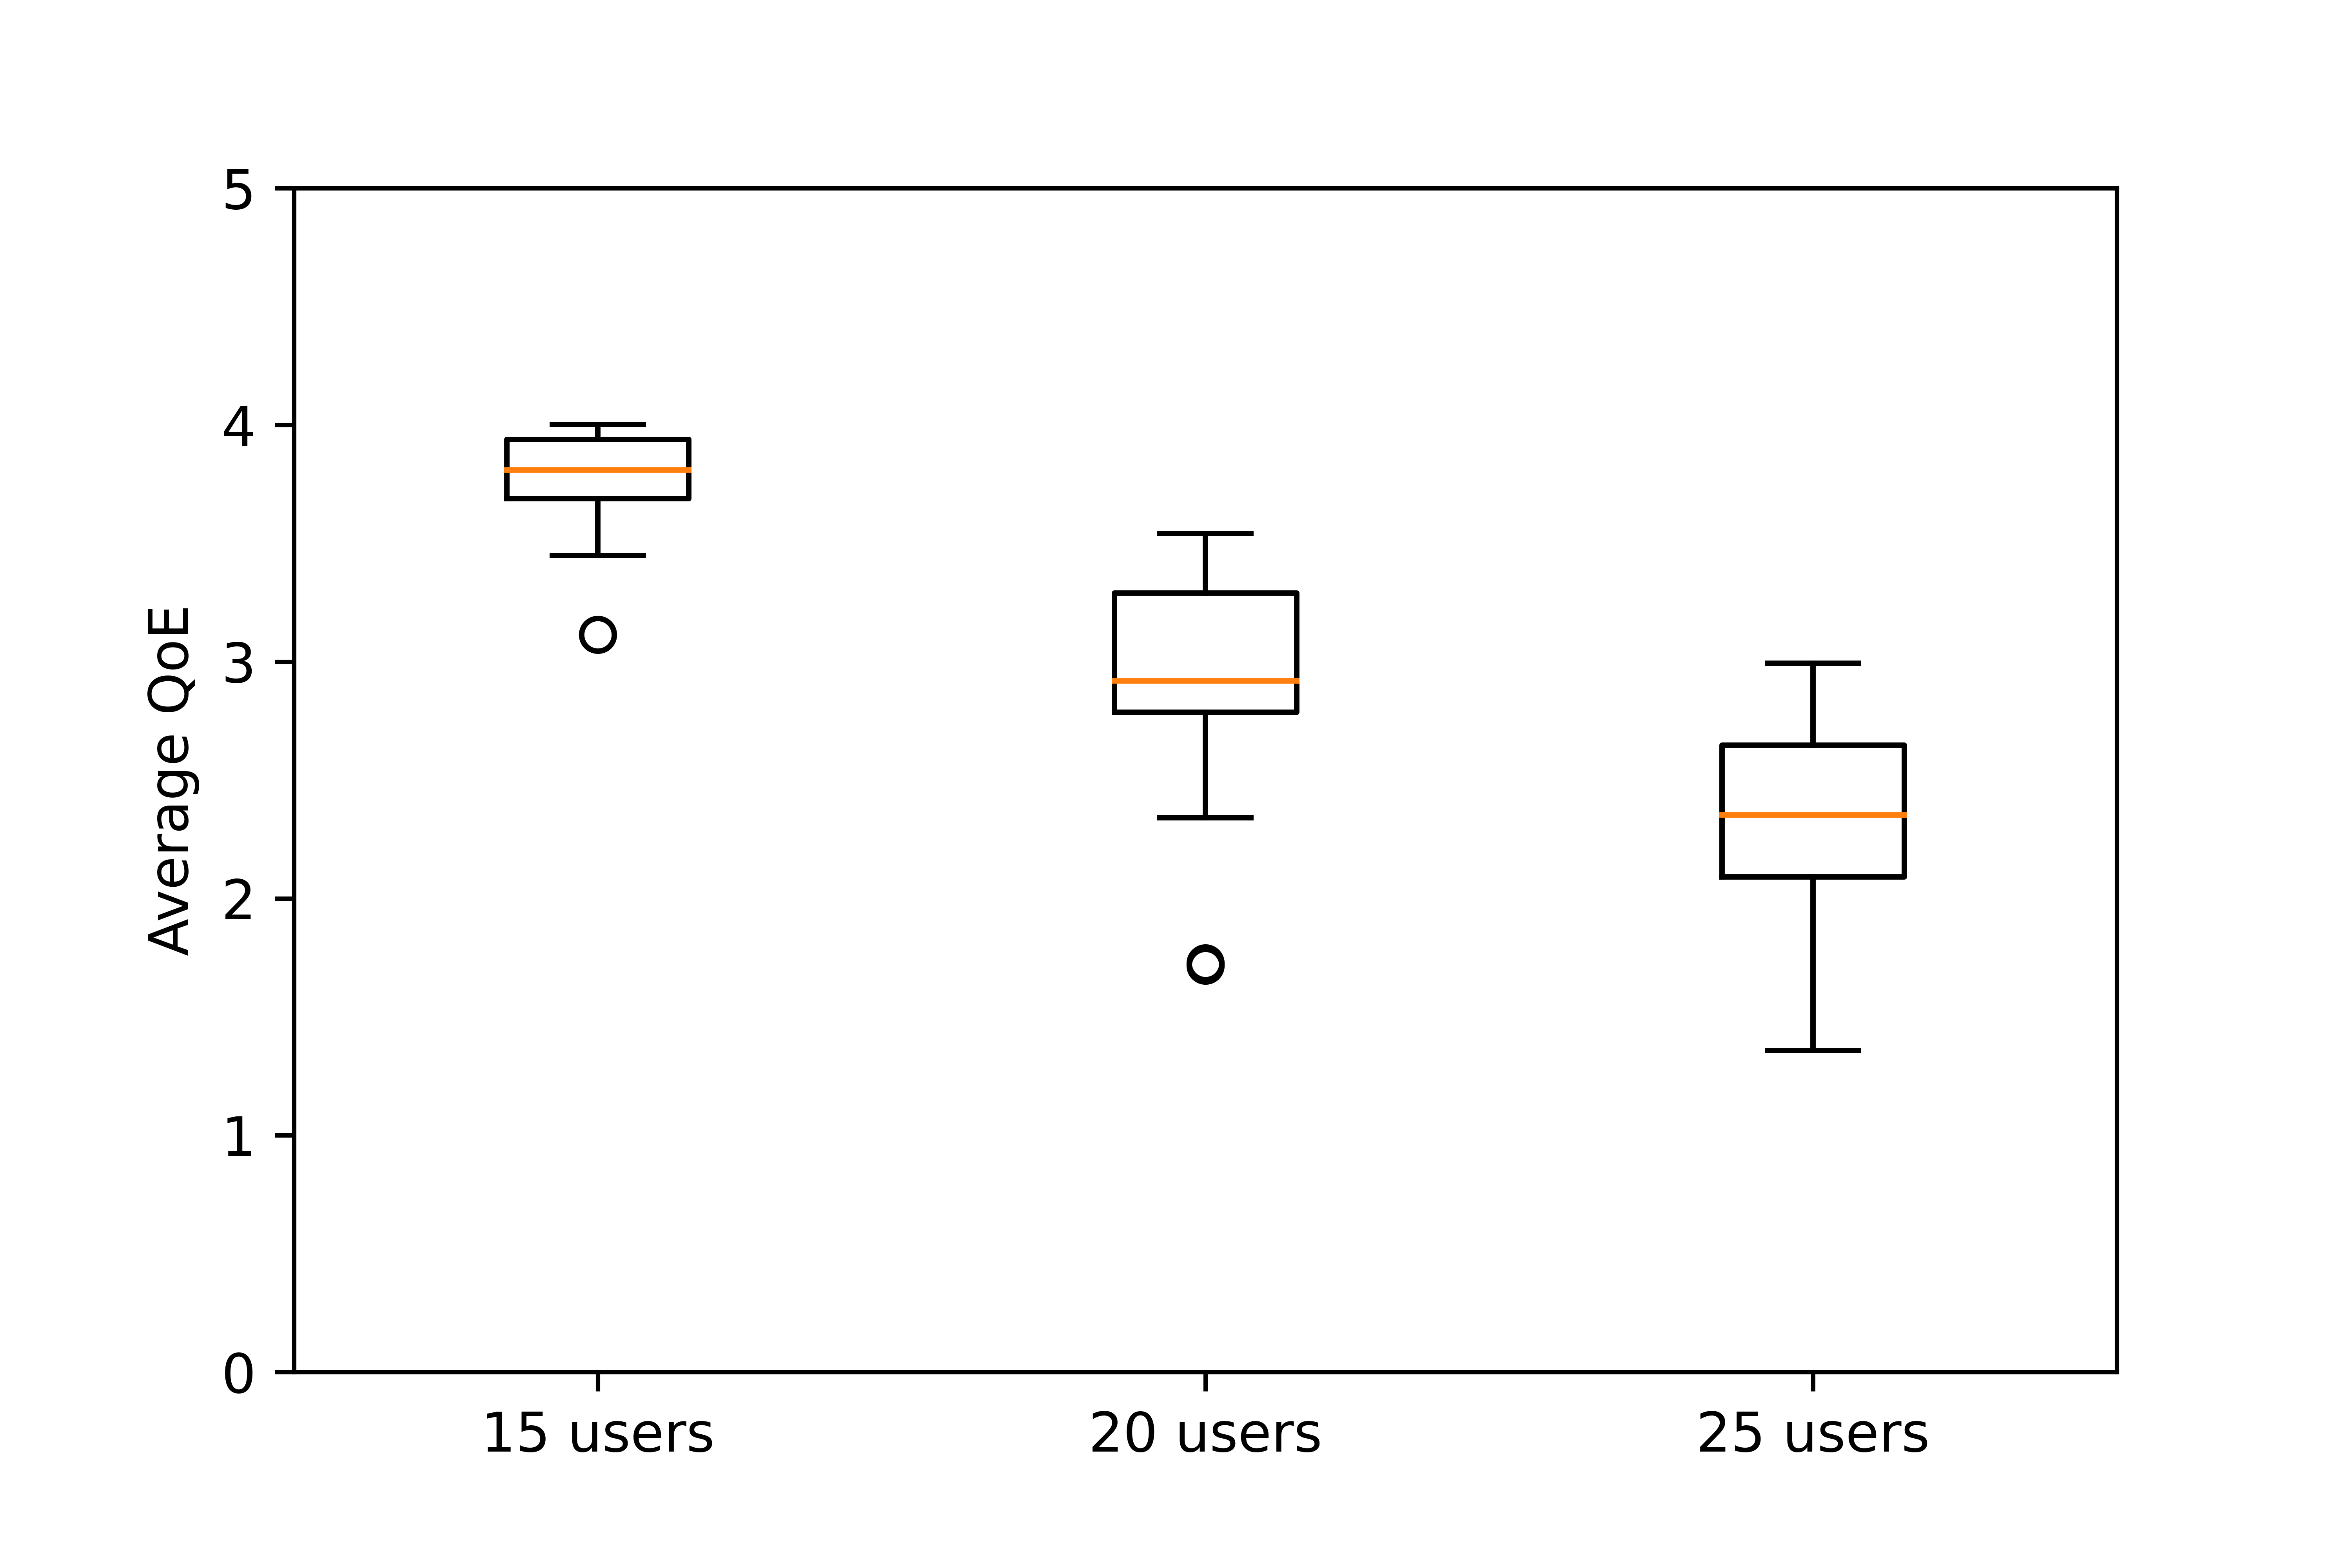
\includegraphics[width=0.45\linewidth]{images/QoEBoxplot.png}
%     \label{fig:co-comparison-boxplot}
%     }

%     \subfigure[]{
%     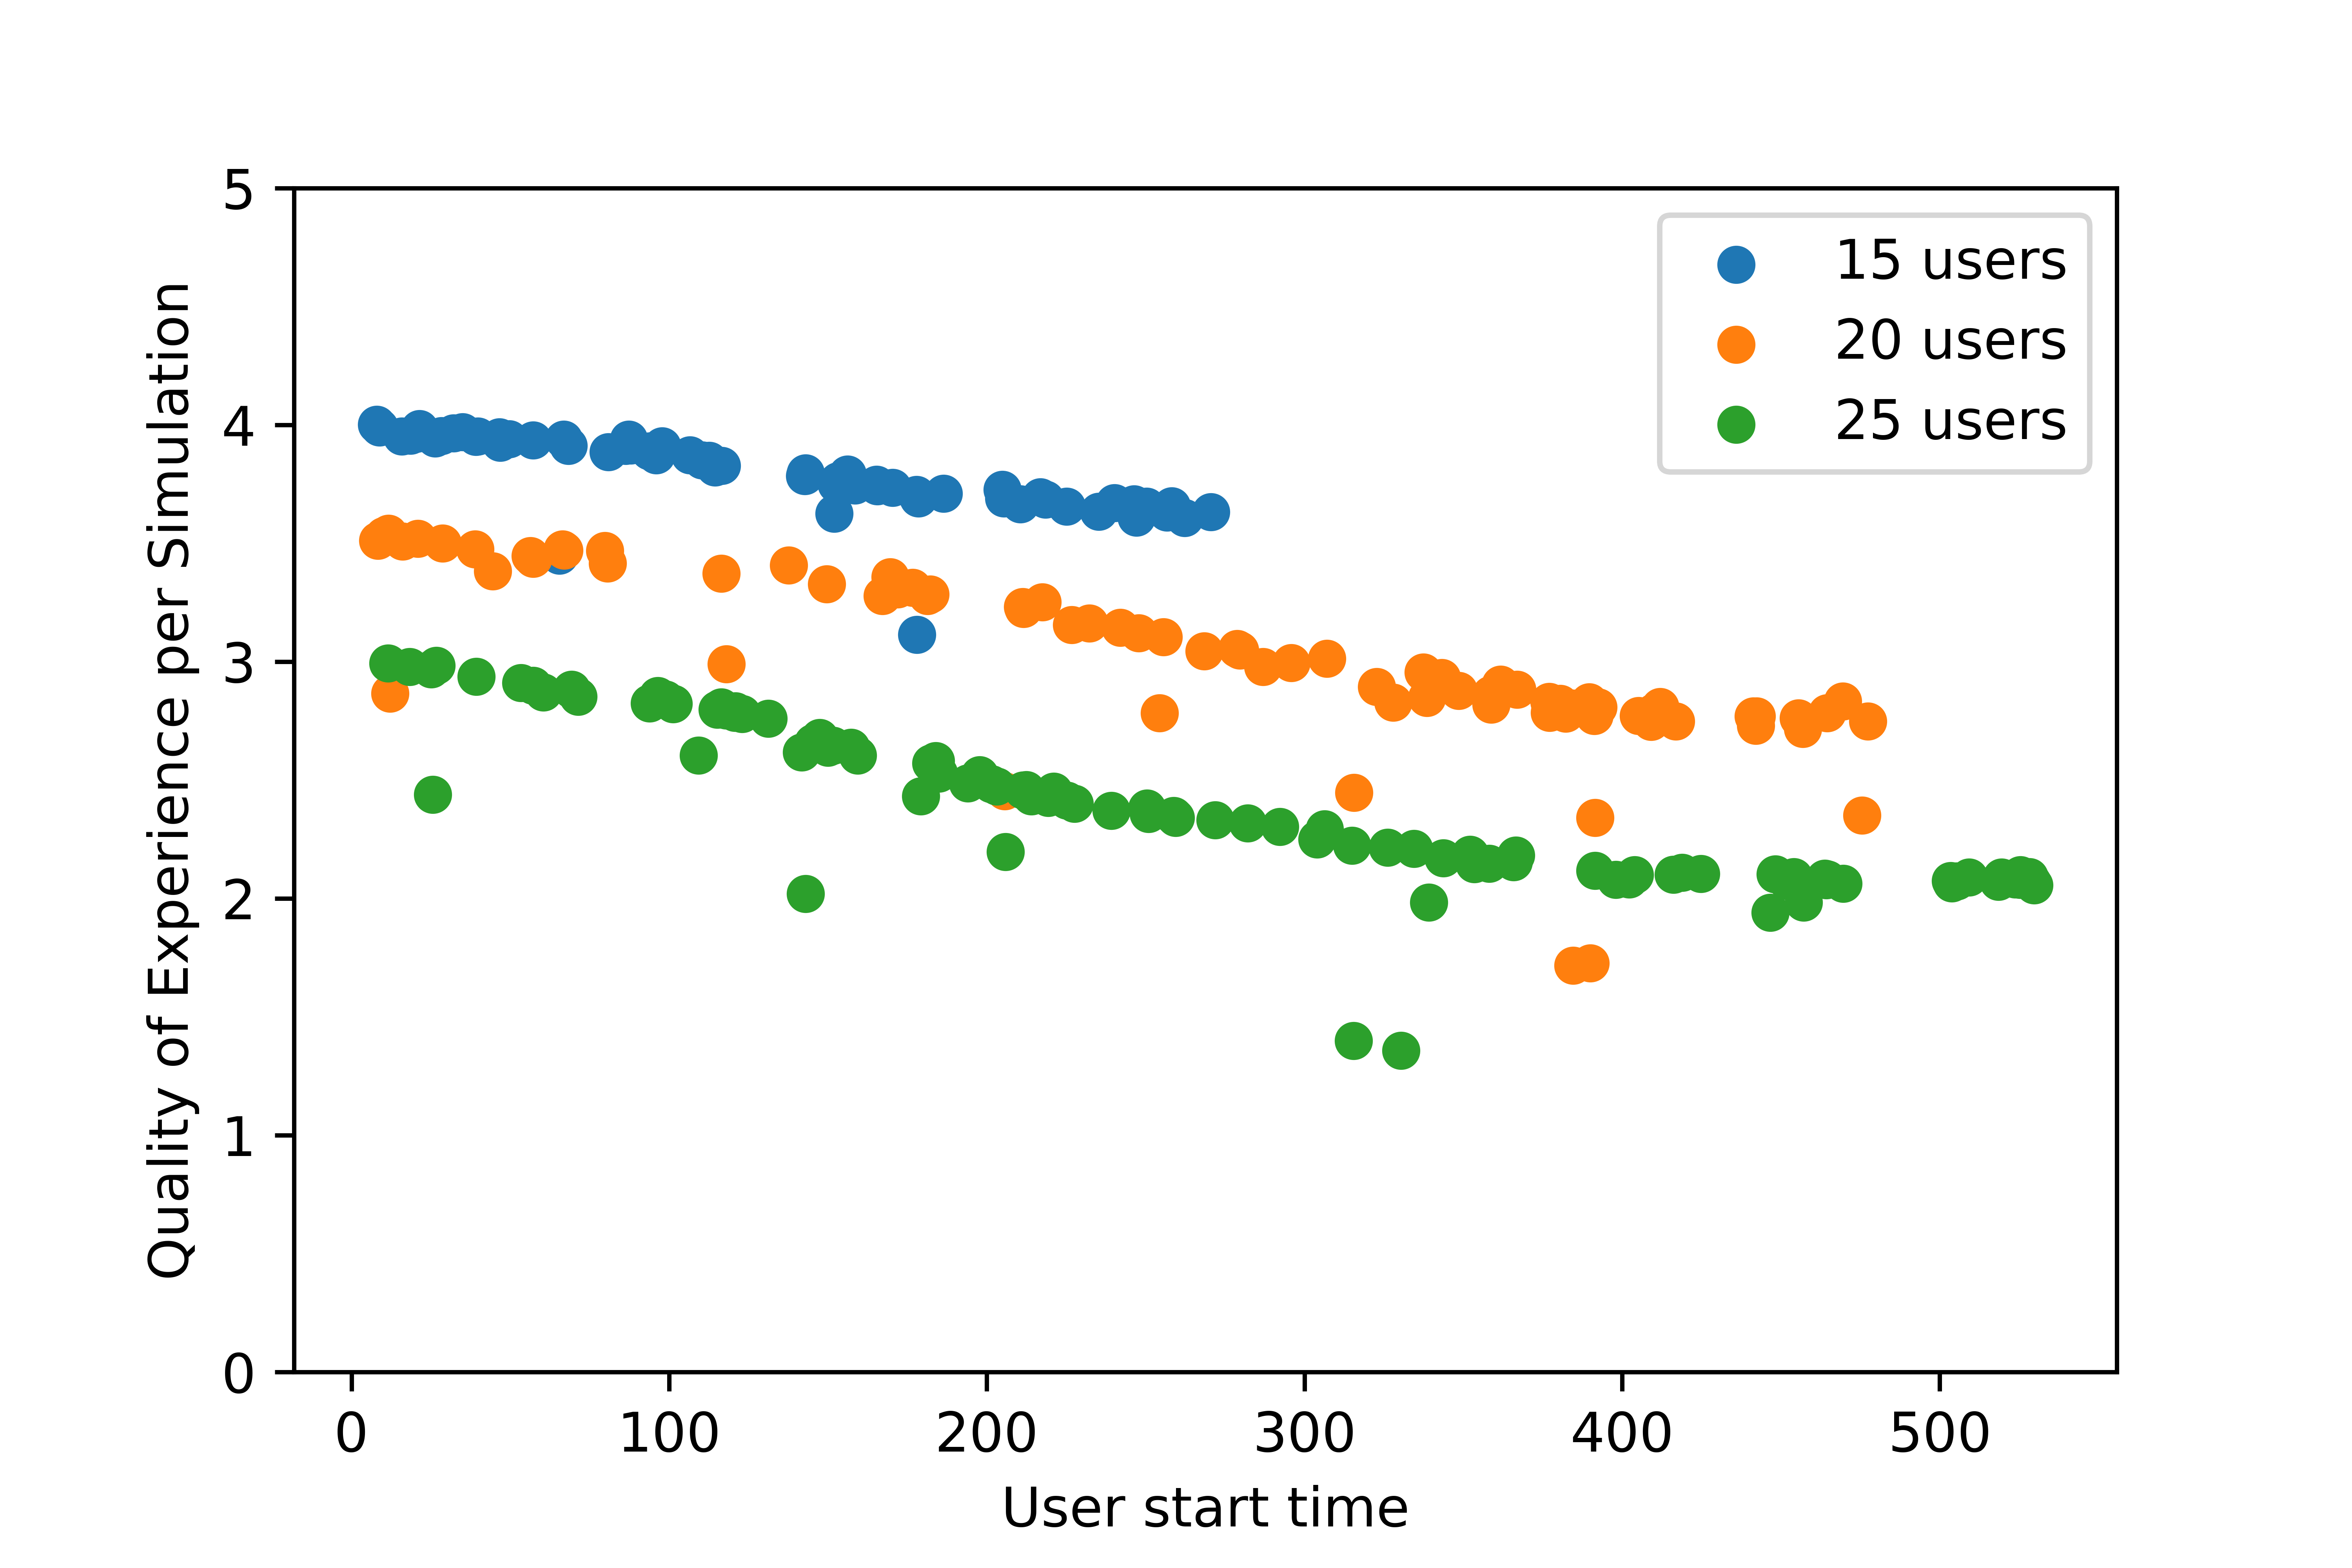
\includegraphics[width=0.45\linewidth]{images/QoECompare.png}
%     \label{fig:red-comparison-plot}
%     }
%     \subfigure[]{
%     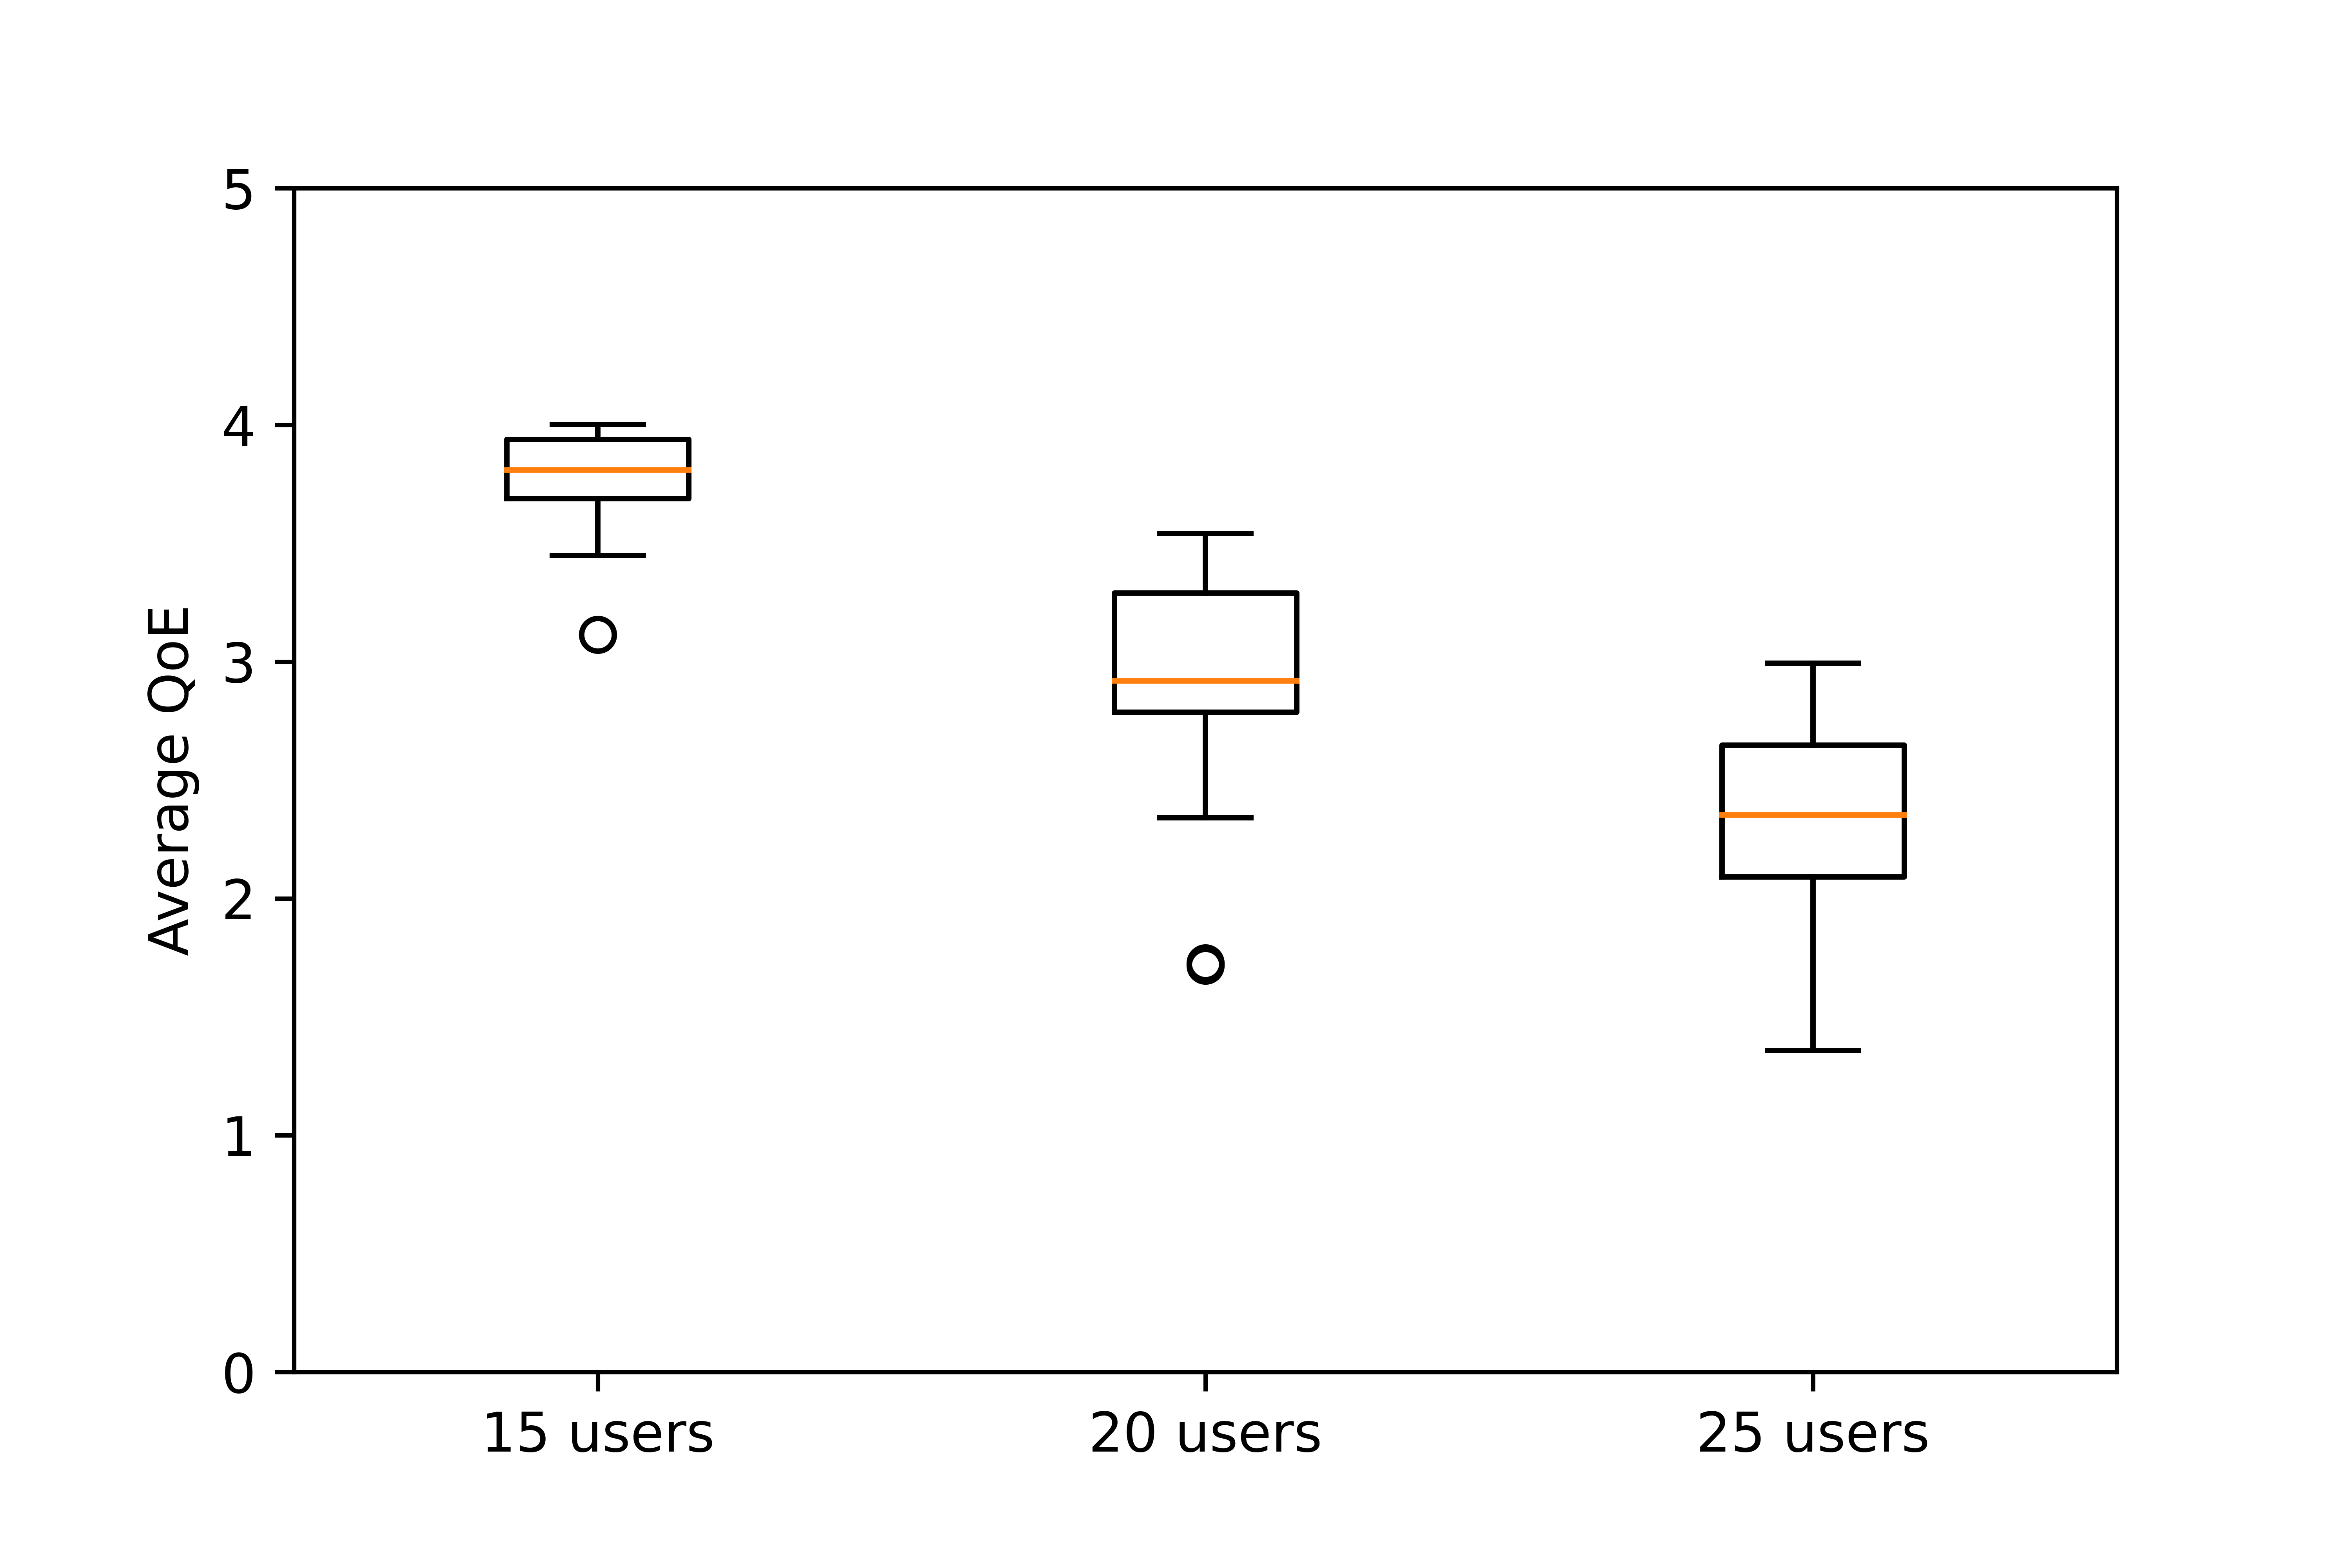
\includegraphics[width=0.45\linewidth]{images/QoEBoxplot.png}
%     \label{fig:red-comparison-boxplot}
%     }

%     \caption{Impact of system on the network performance. Distance \textit{d} between sensor node and antennas of 8m in a semi-NLOS scenario.}
%     \label{fig:comparison-rof-2}
% \end{figure*}

\begin{figure*}
    \centering
    \subfigure[]{
    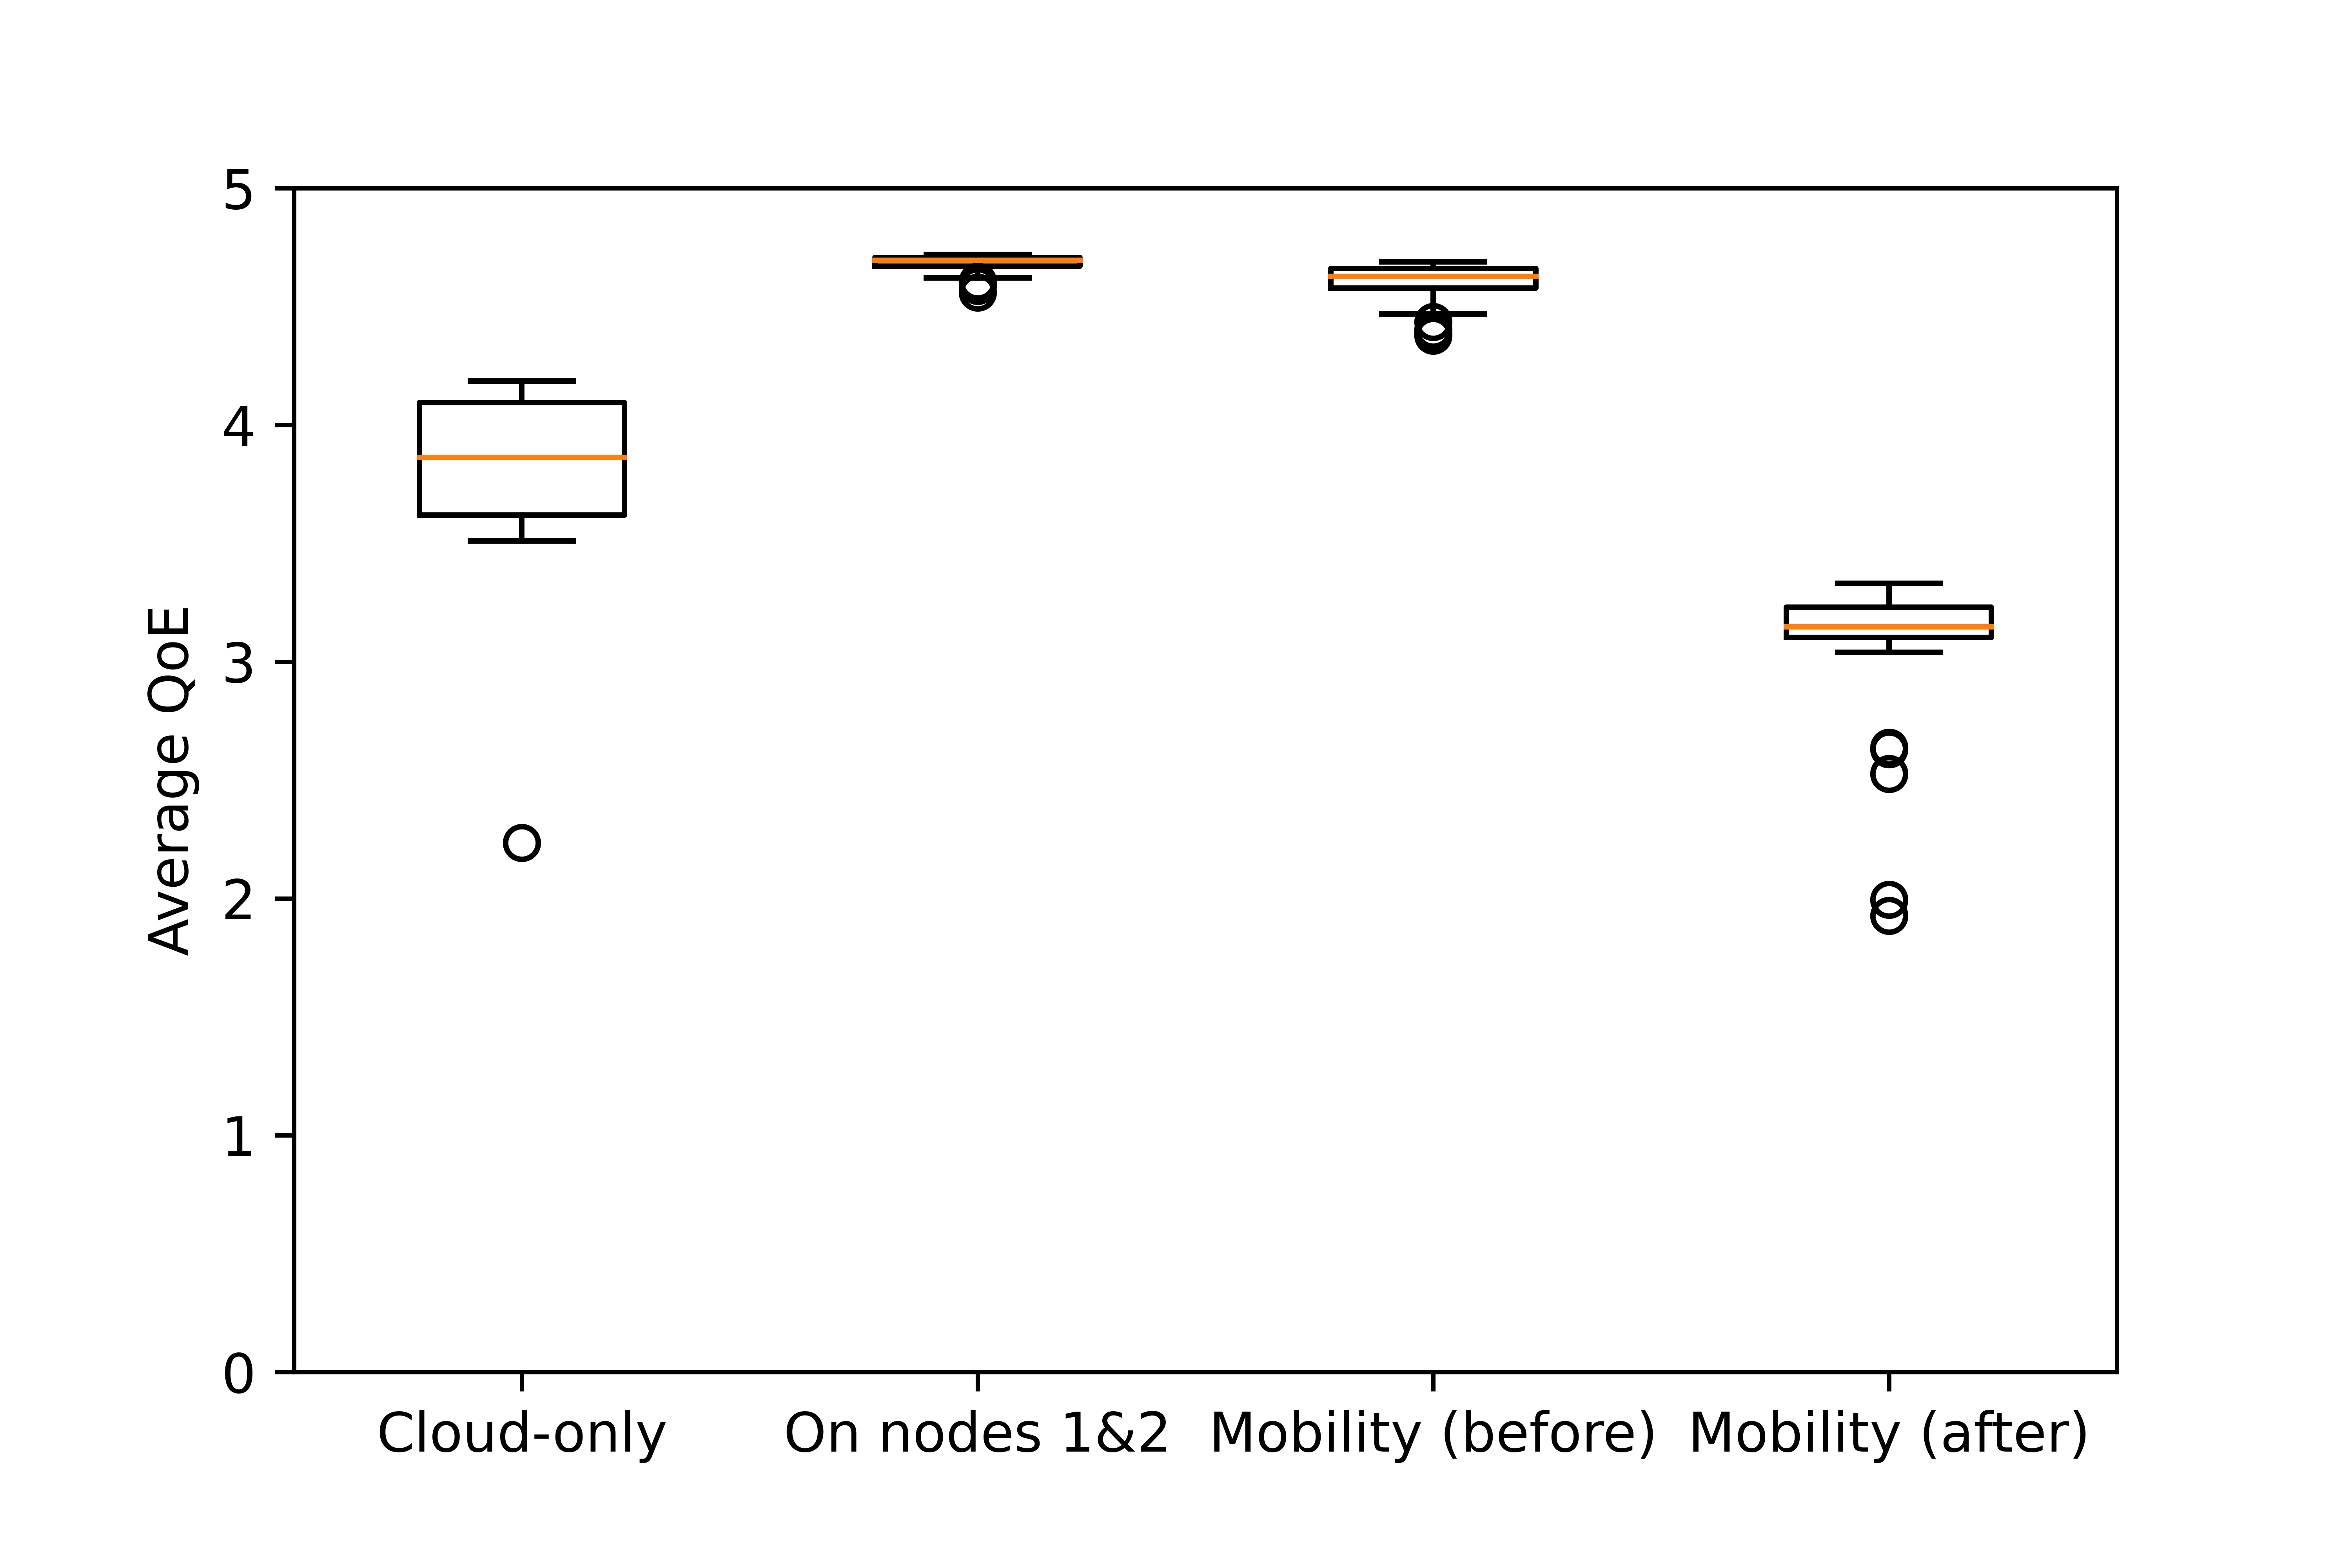
\includegraphics[width=0.31\linewidth]{images/QoEBoxplot-15u.png}
    \label{fig:red-comparison-plot}
    }
    \subfigure[]{
    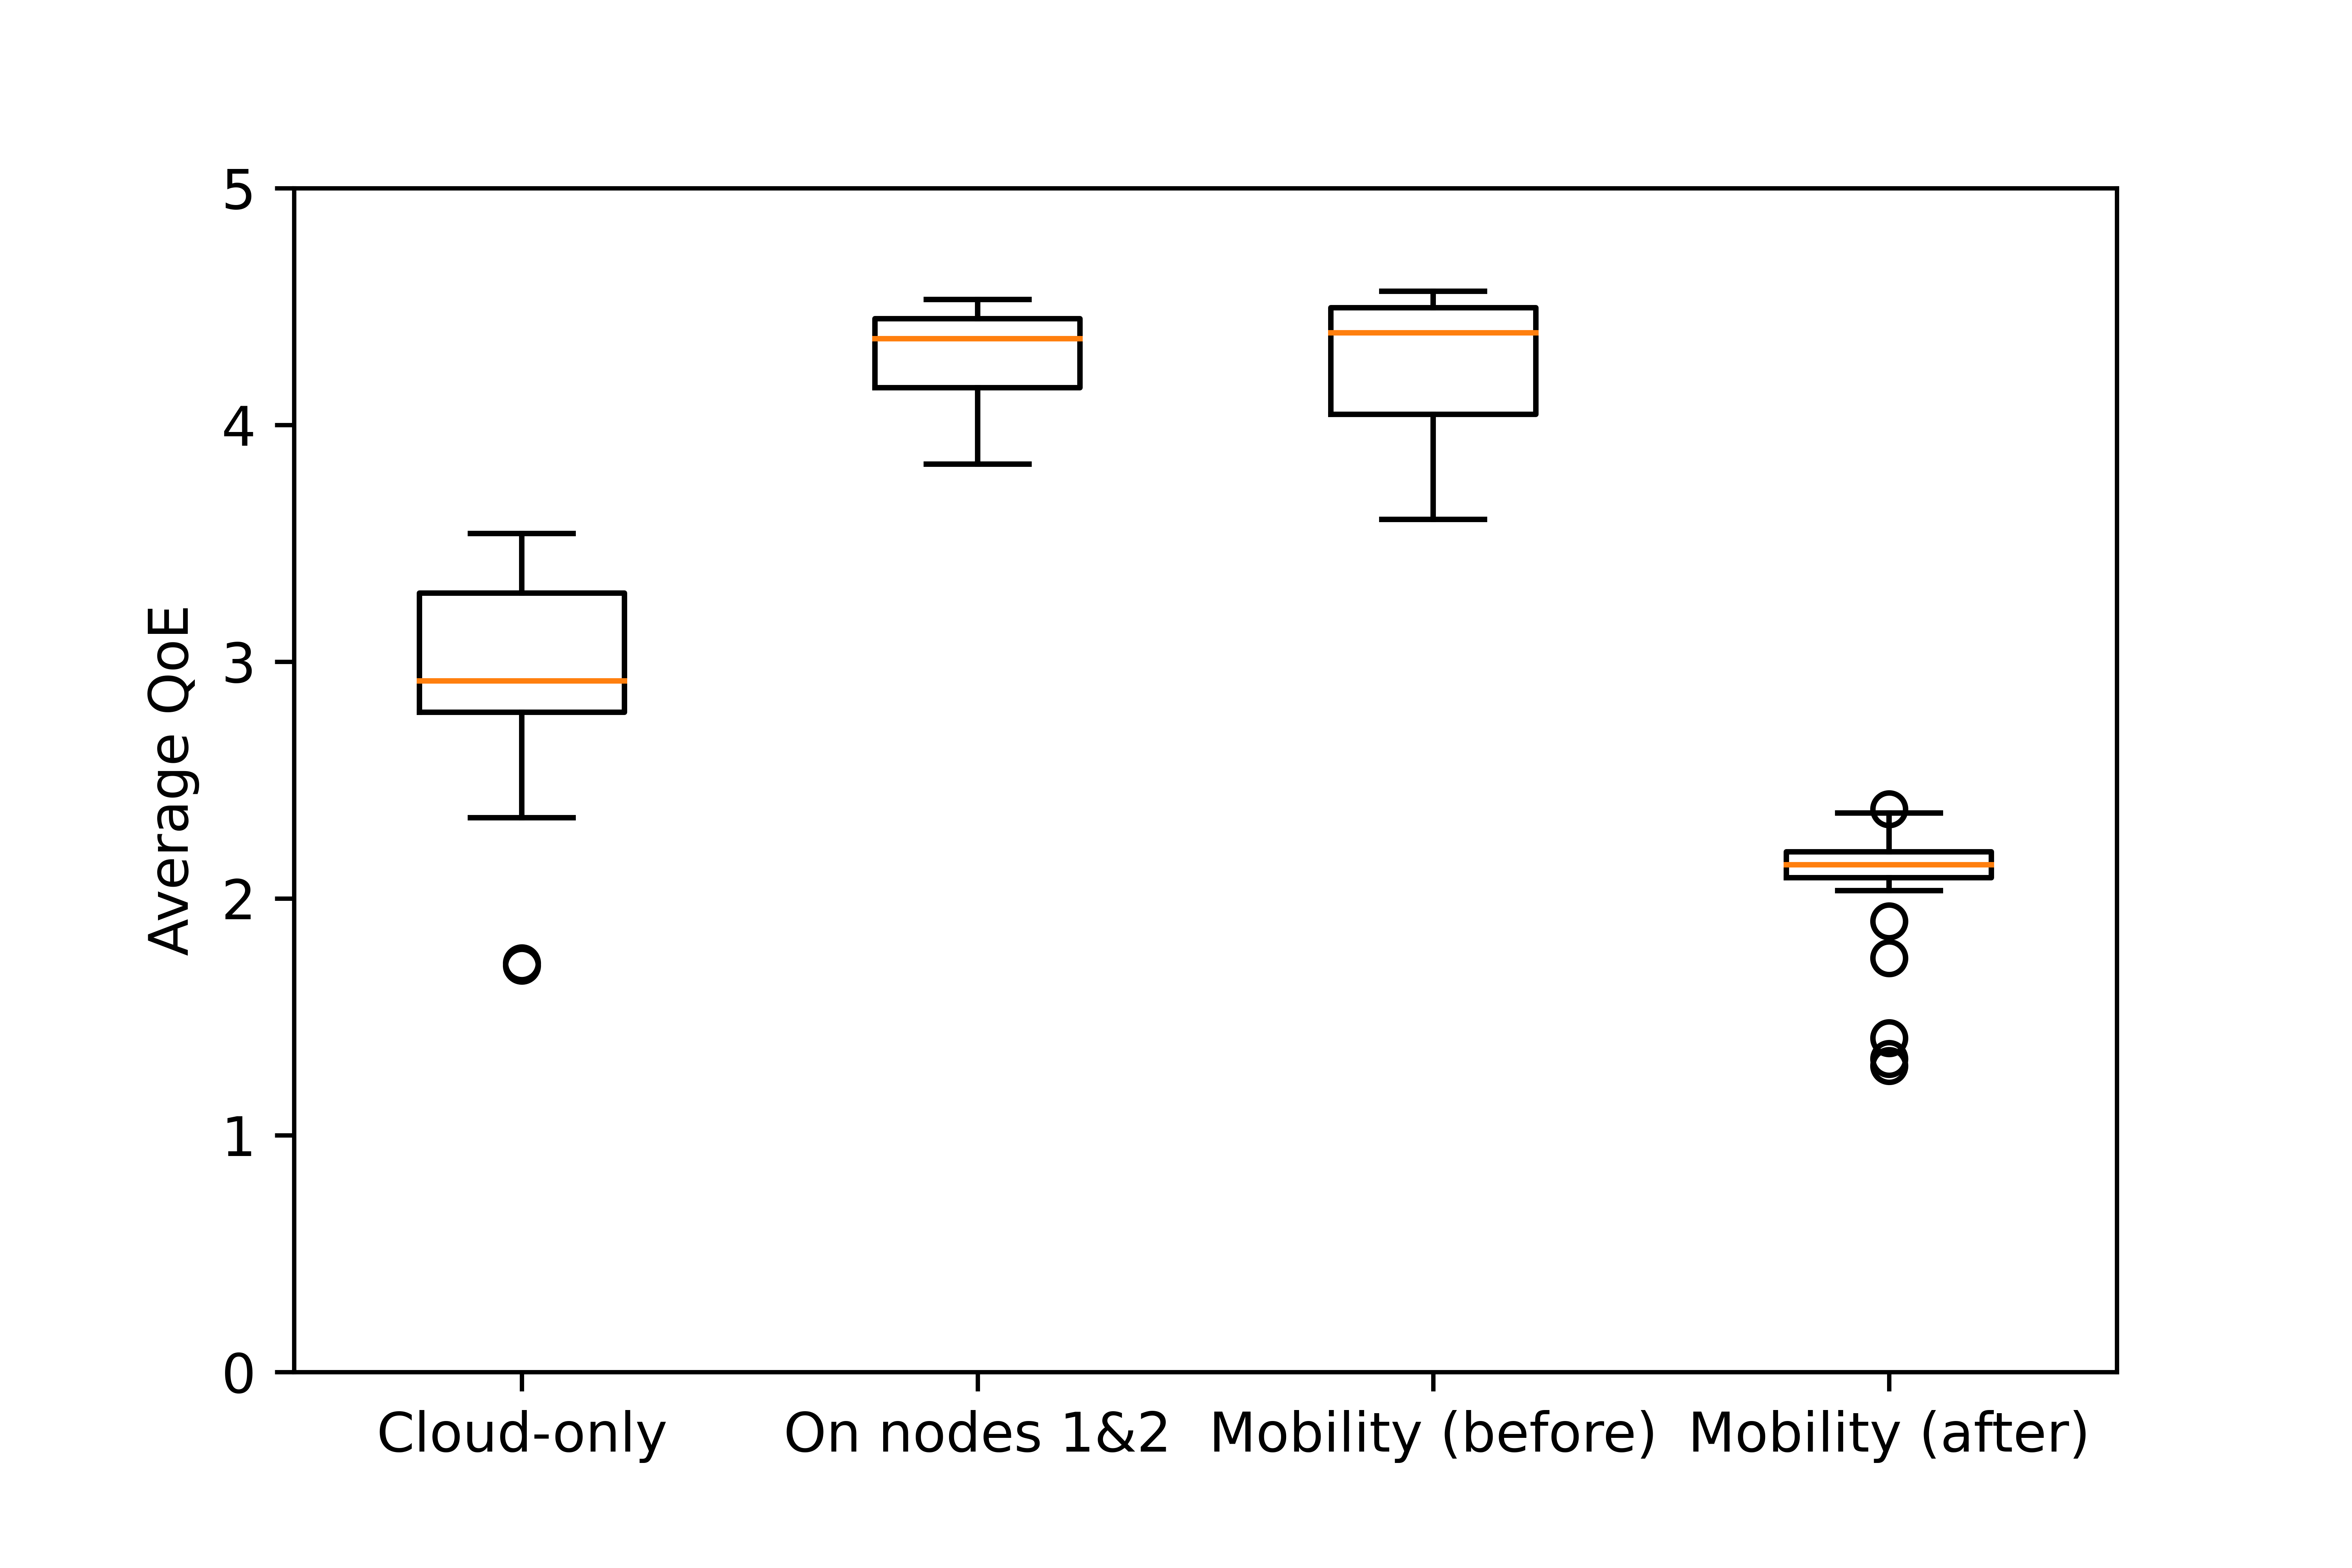
\includegraphics[width=0.31\linewidth]{images/QoEBoxplot-20u.png}
    \label{fig:co-comparison-boxplot}
    }
    \subfigure[]{
    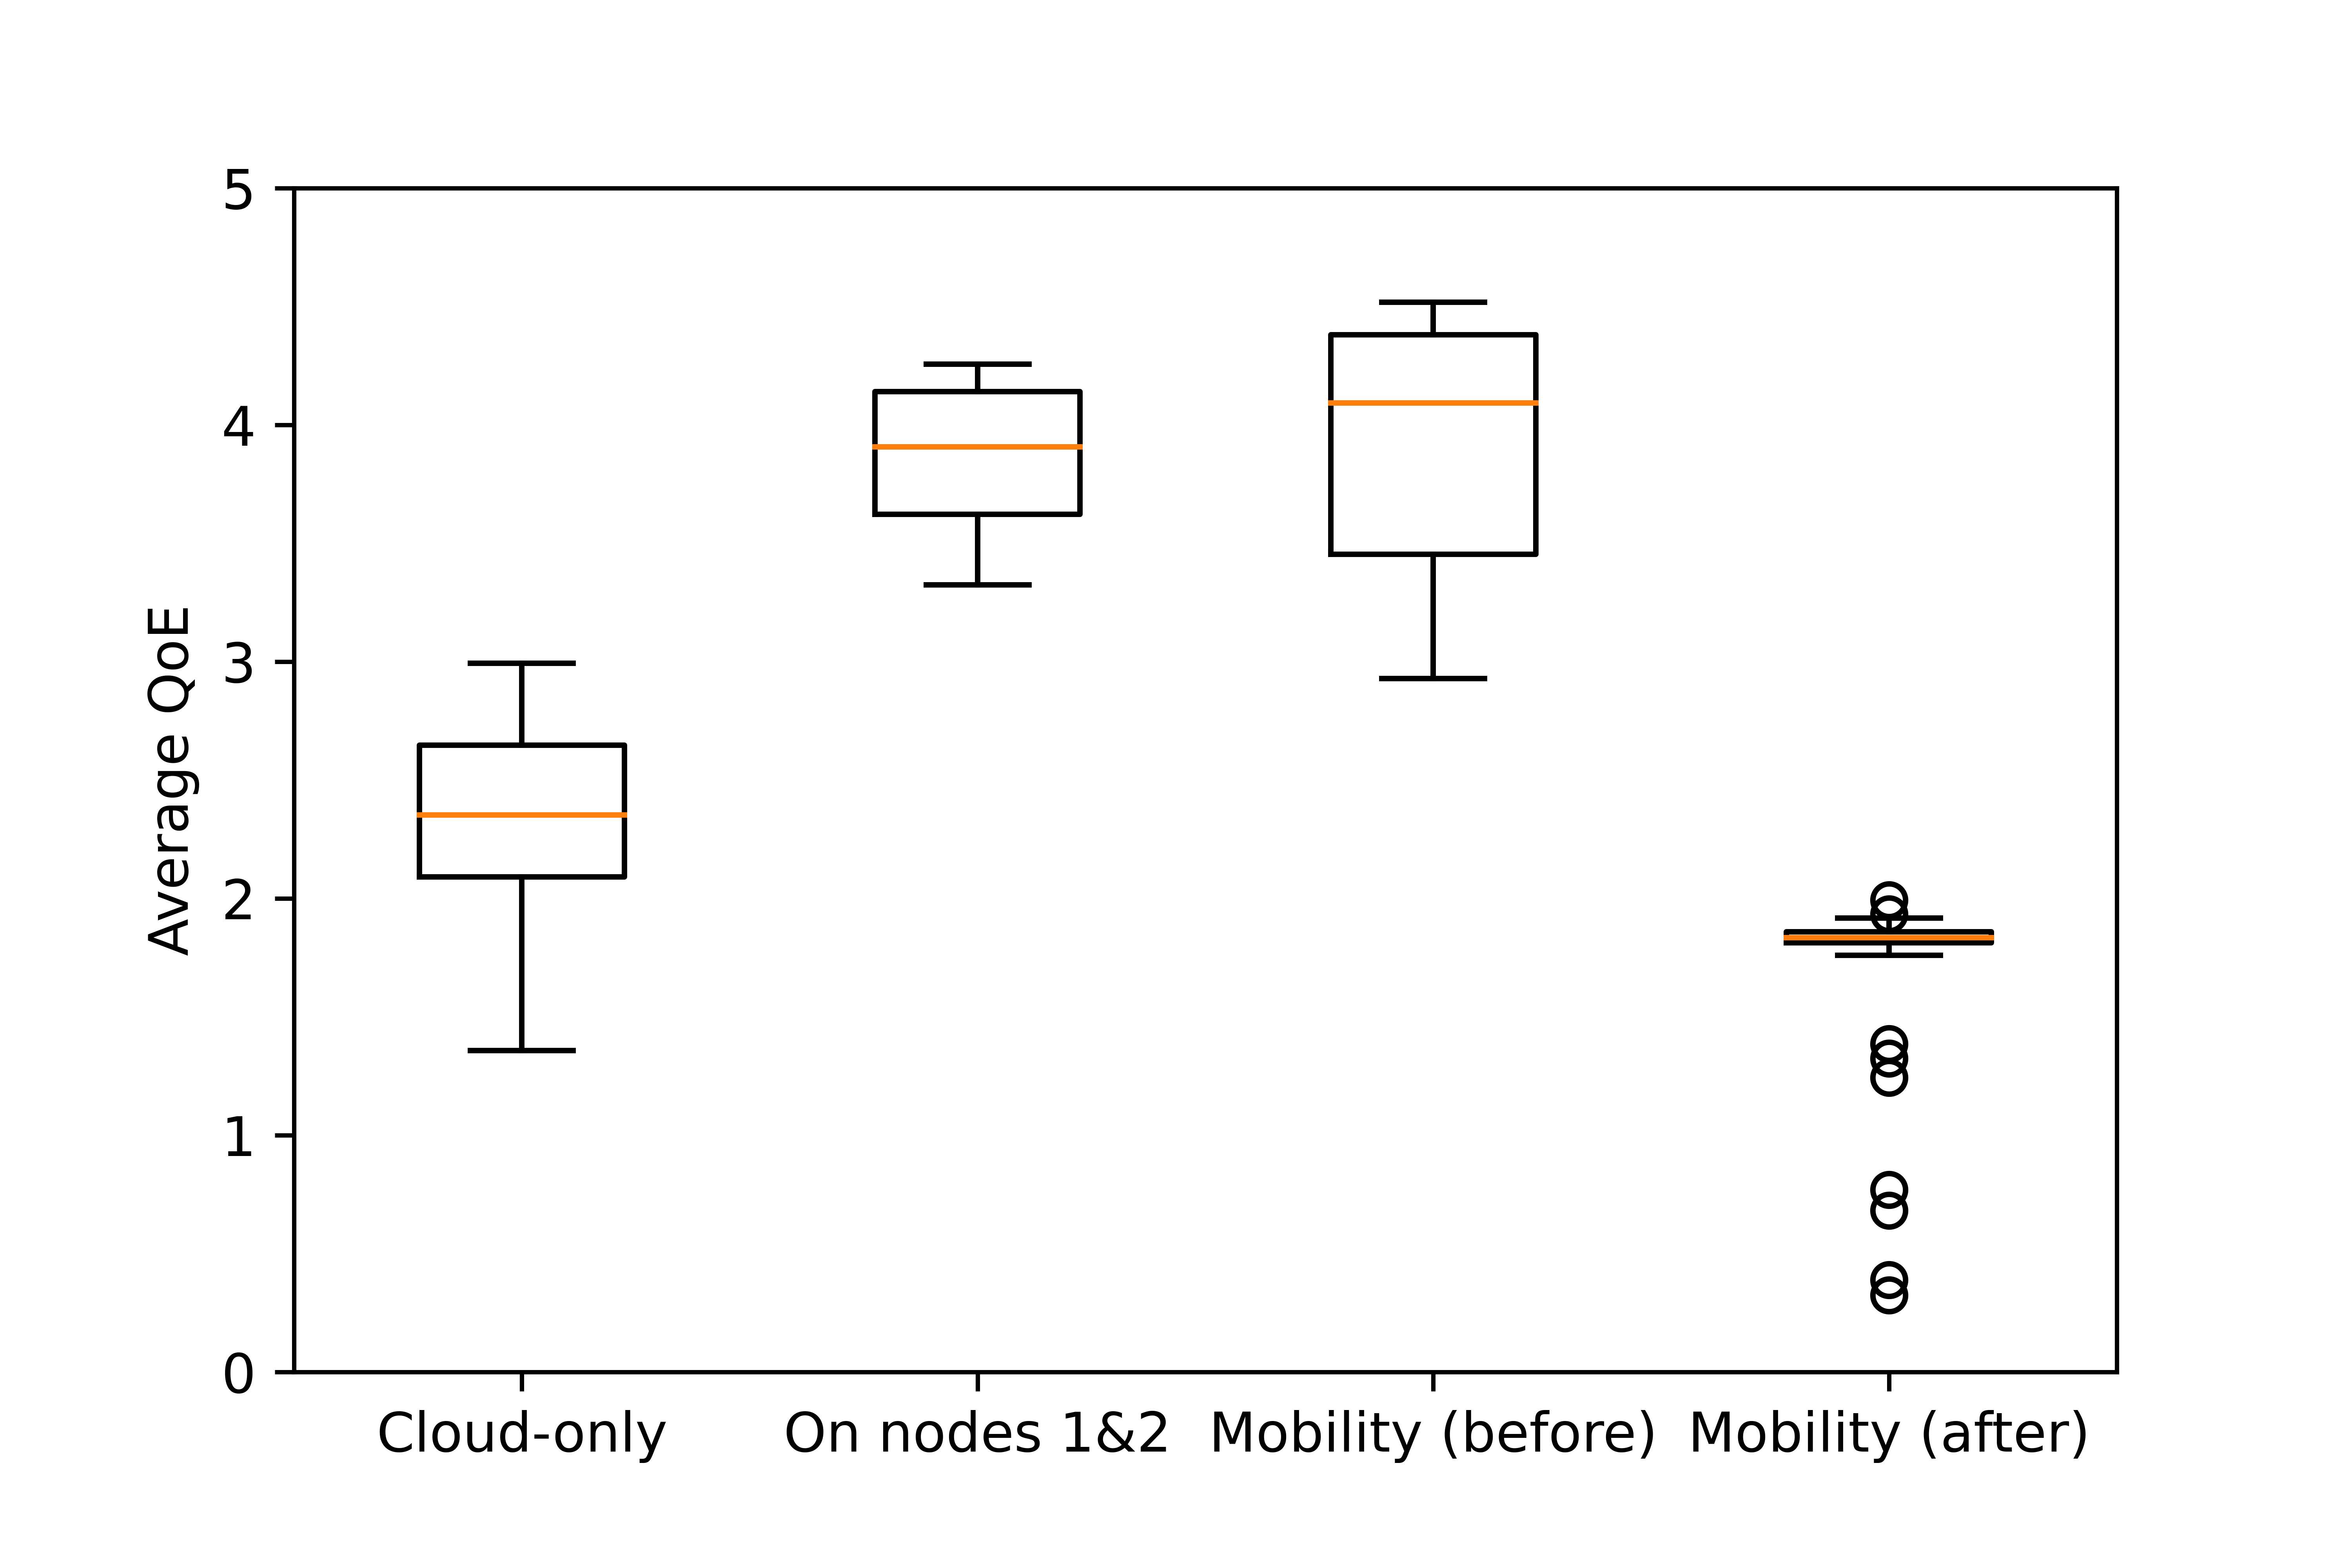
\includegraphics[width=0.31\linewidth]{images/QoEBoxplot-25u.png}
    \label{fig:red-comparison-plot}
    }
    
    \caption{Average QoE results for scenarios with 15, 20 and 25 users per AP.}
    \label{fig:comparison-rof-2}
\end{figure*}


\begin{figure*}
    \centering
    \subfigure[]{
    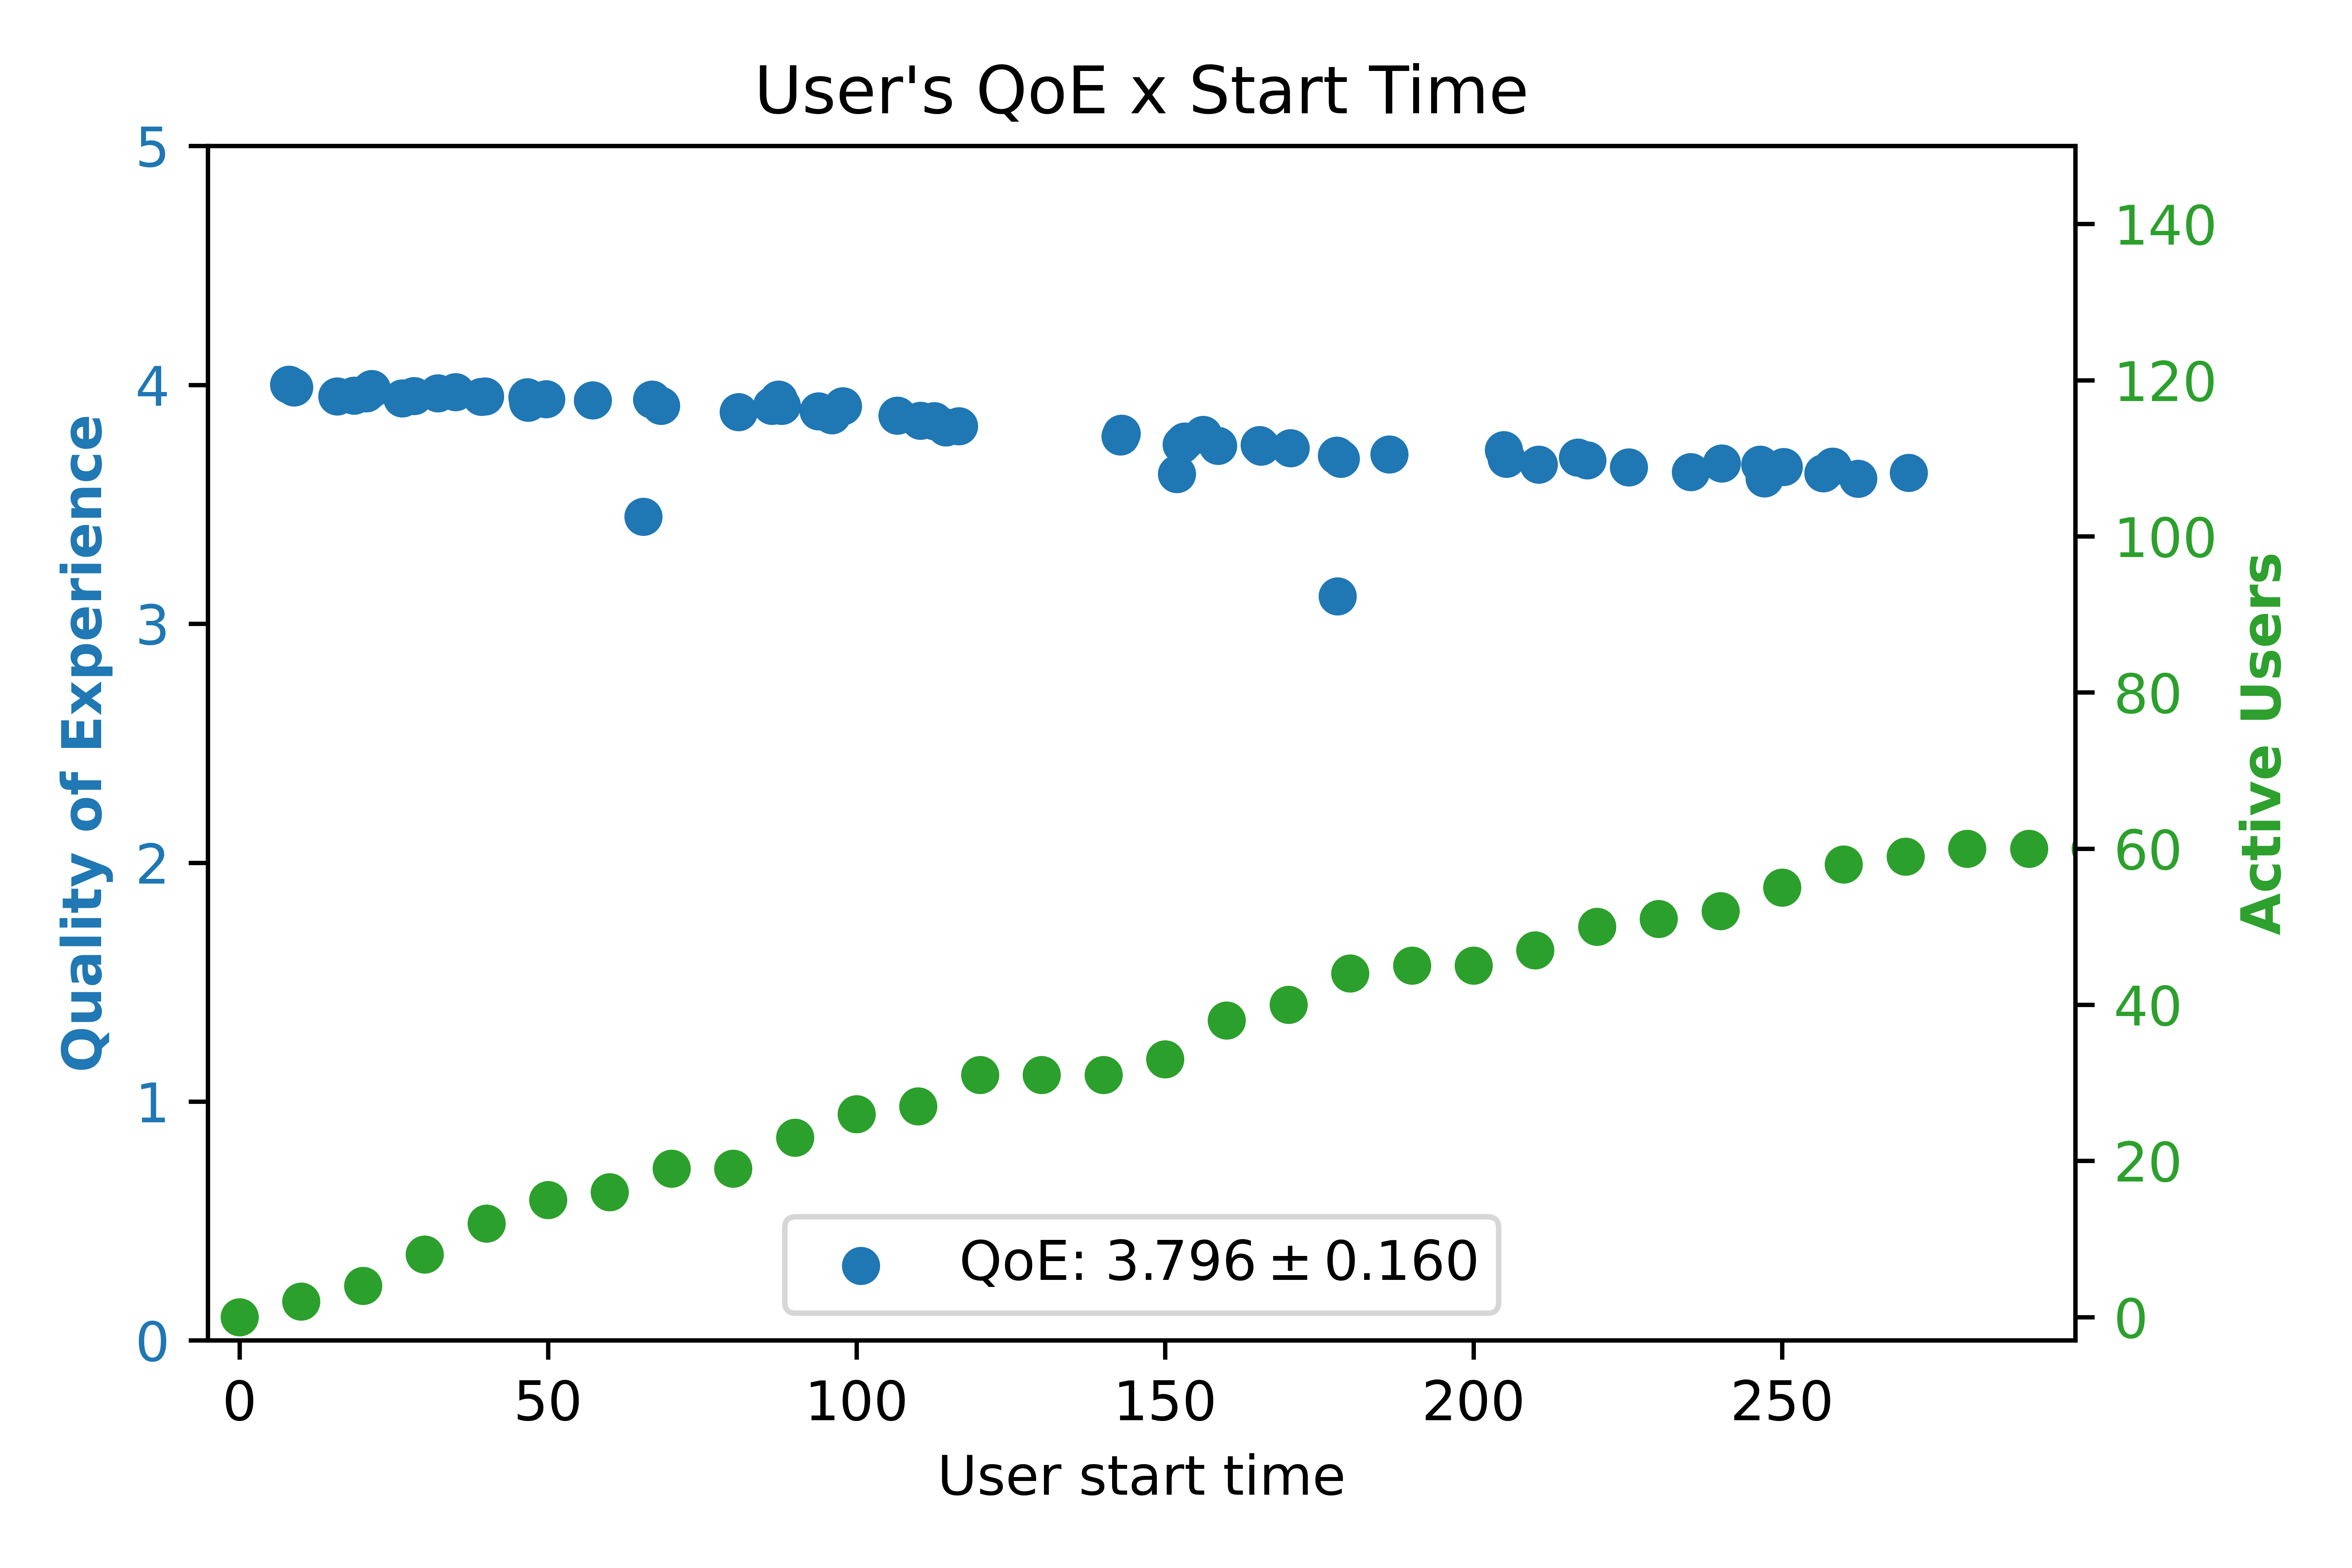
\includegraphics[width=0.31\linewidth]{images/cloud_QoExStartTime15.png}
    \label{fig:rssi-comparison-2}
    }
    \subfigure[]{
    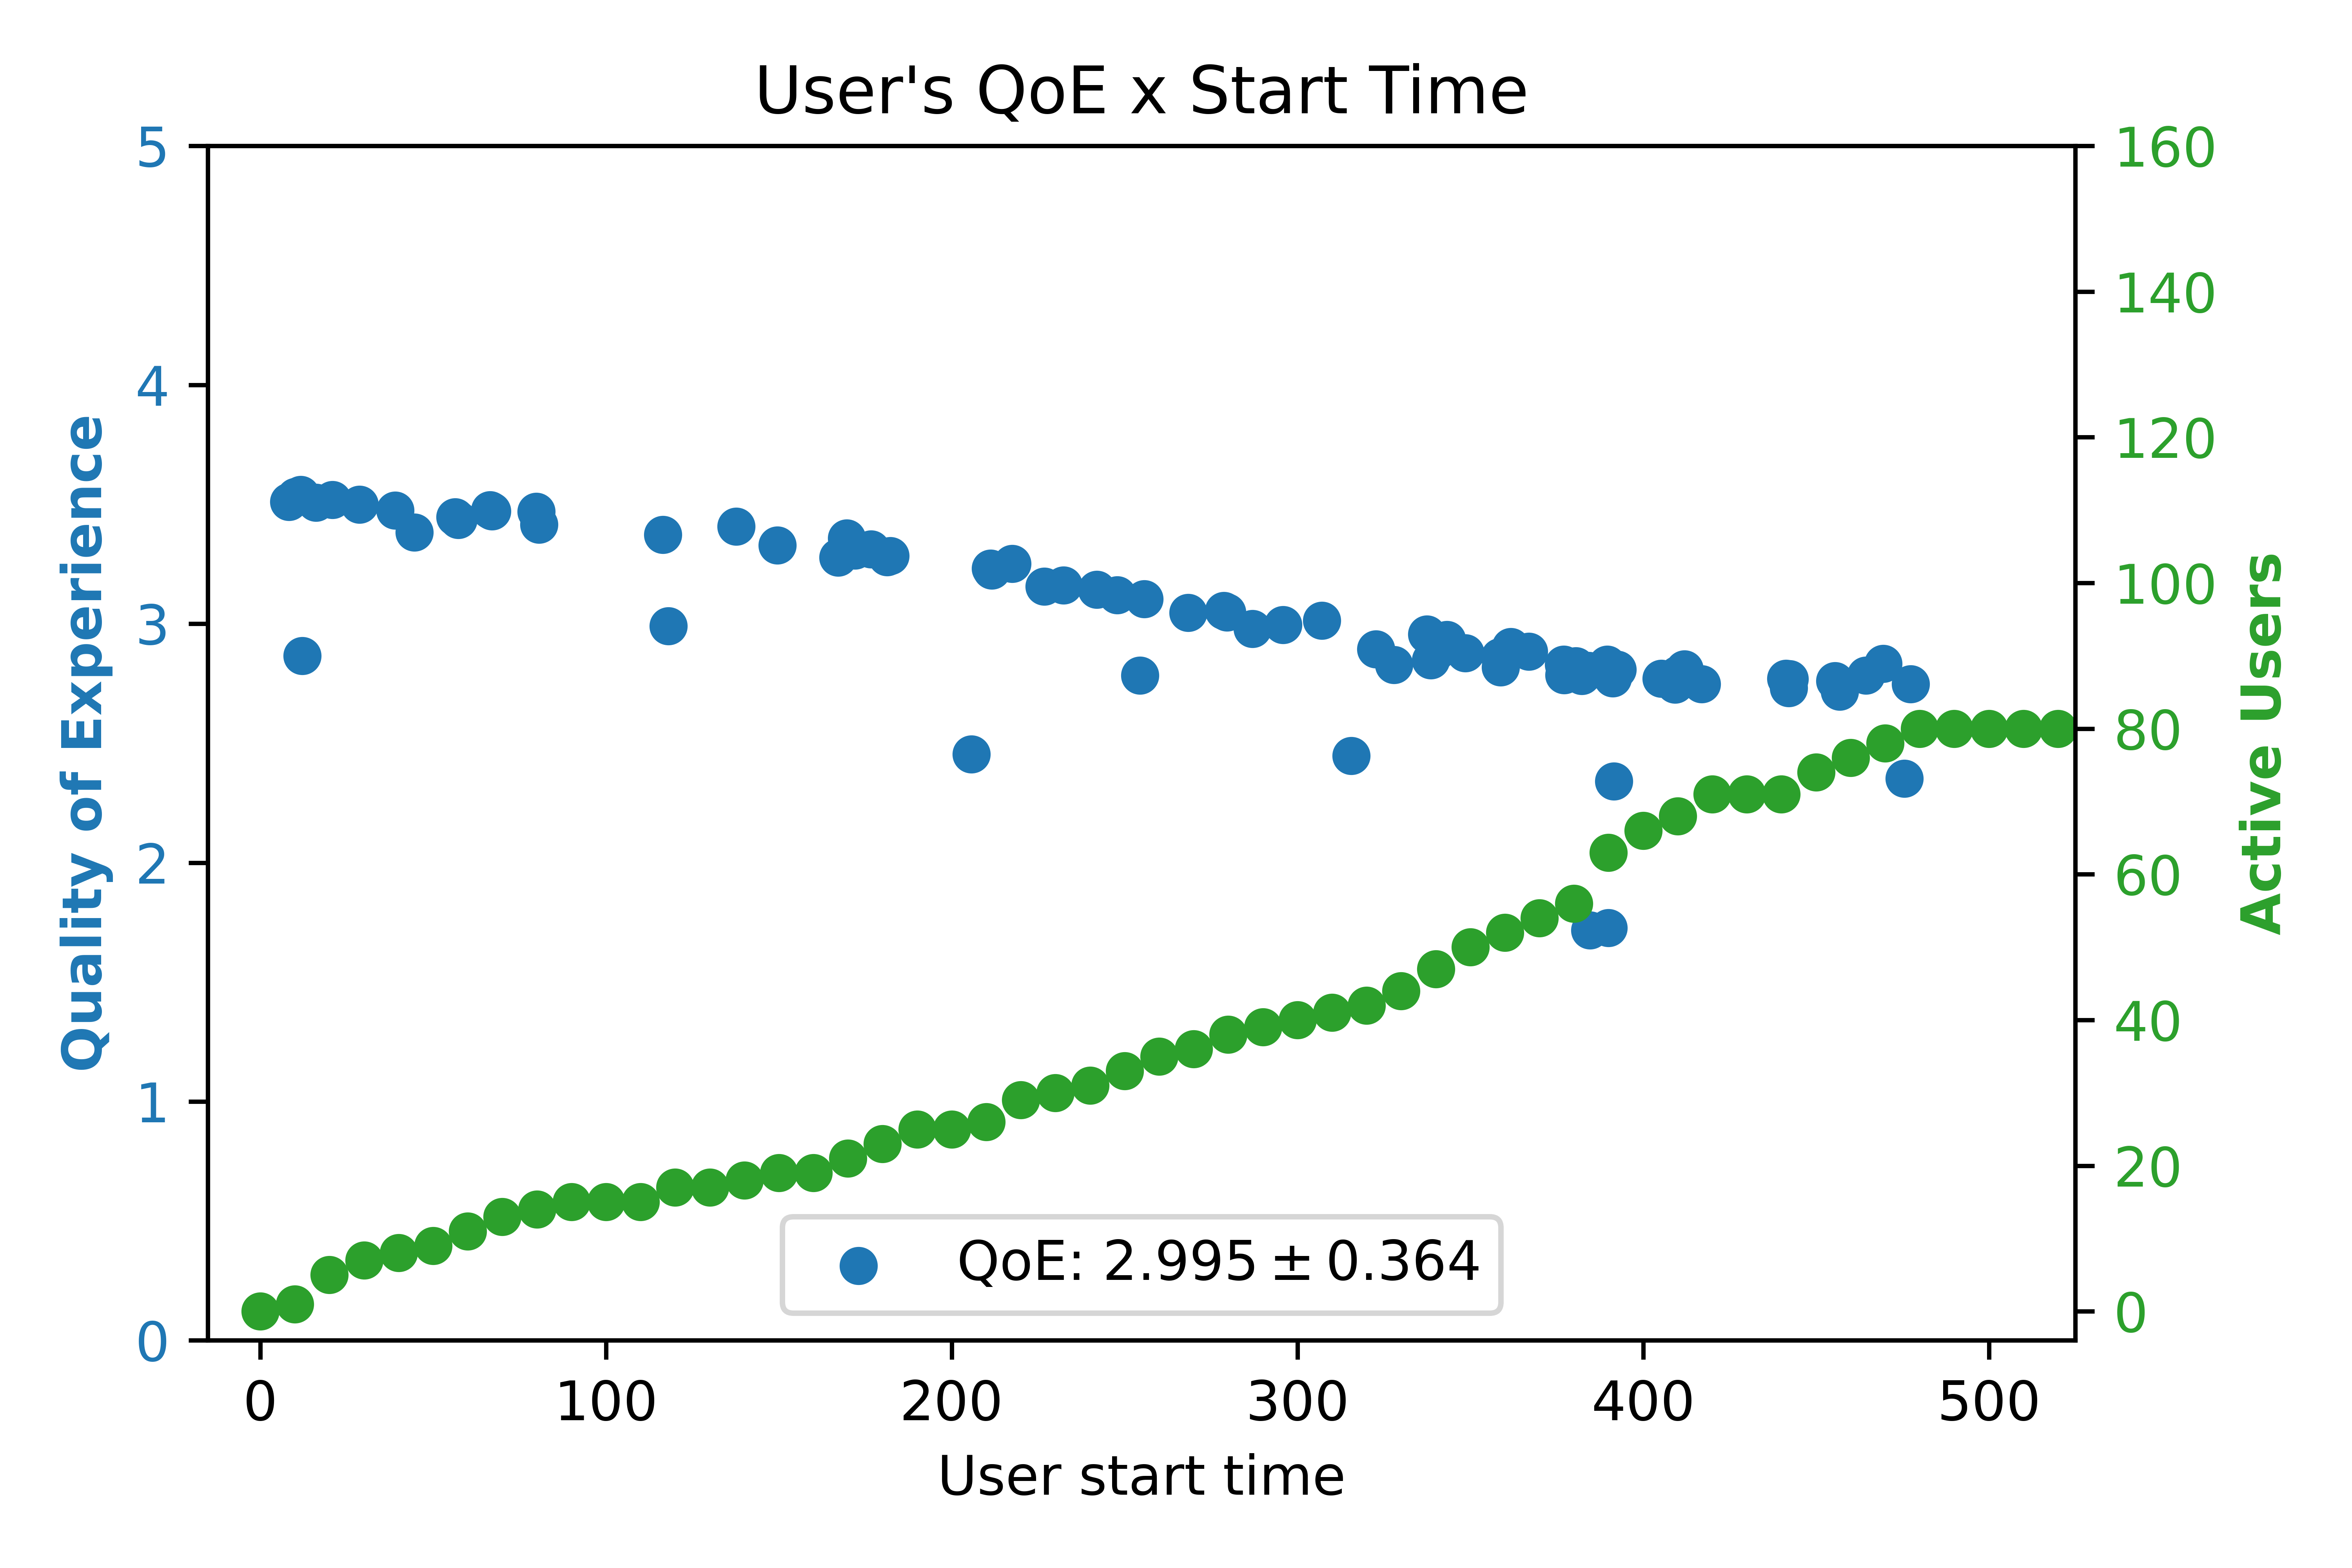
\includegraphics[width=0.31\linewidth]{images/cloud_QoExStartTime20.png}
    \label{fig:plr-comparison-2}
    }
    \subfigure[]{
    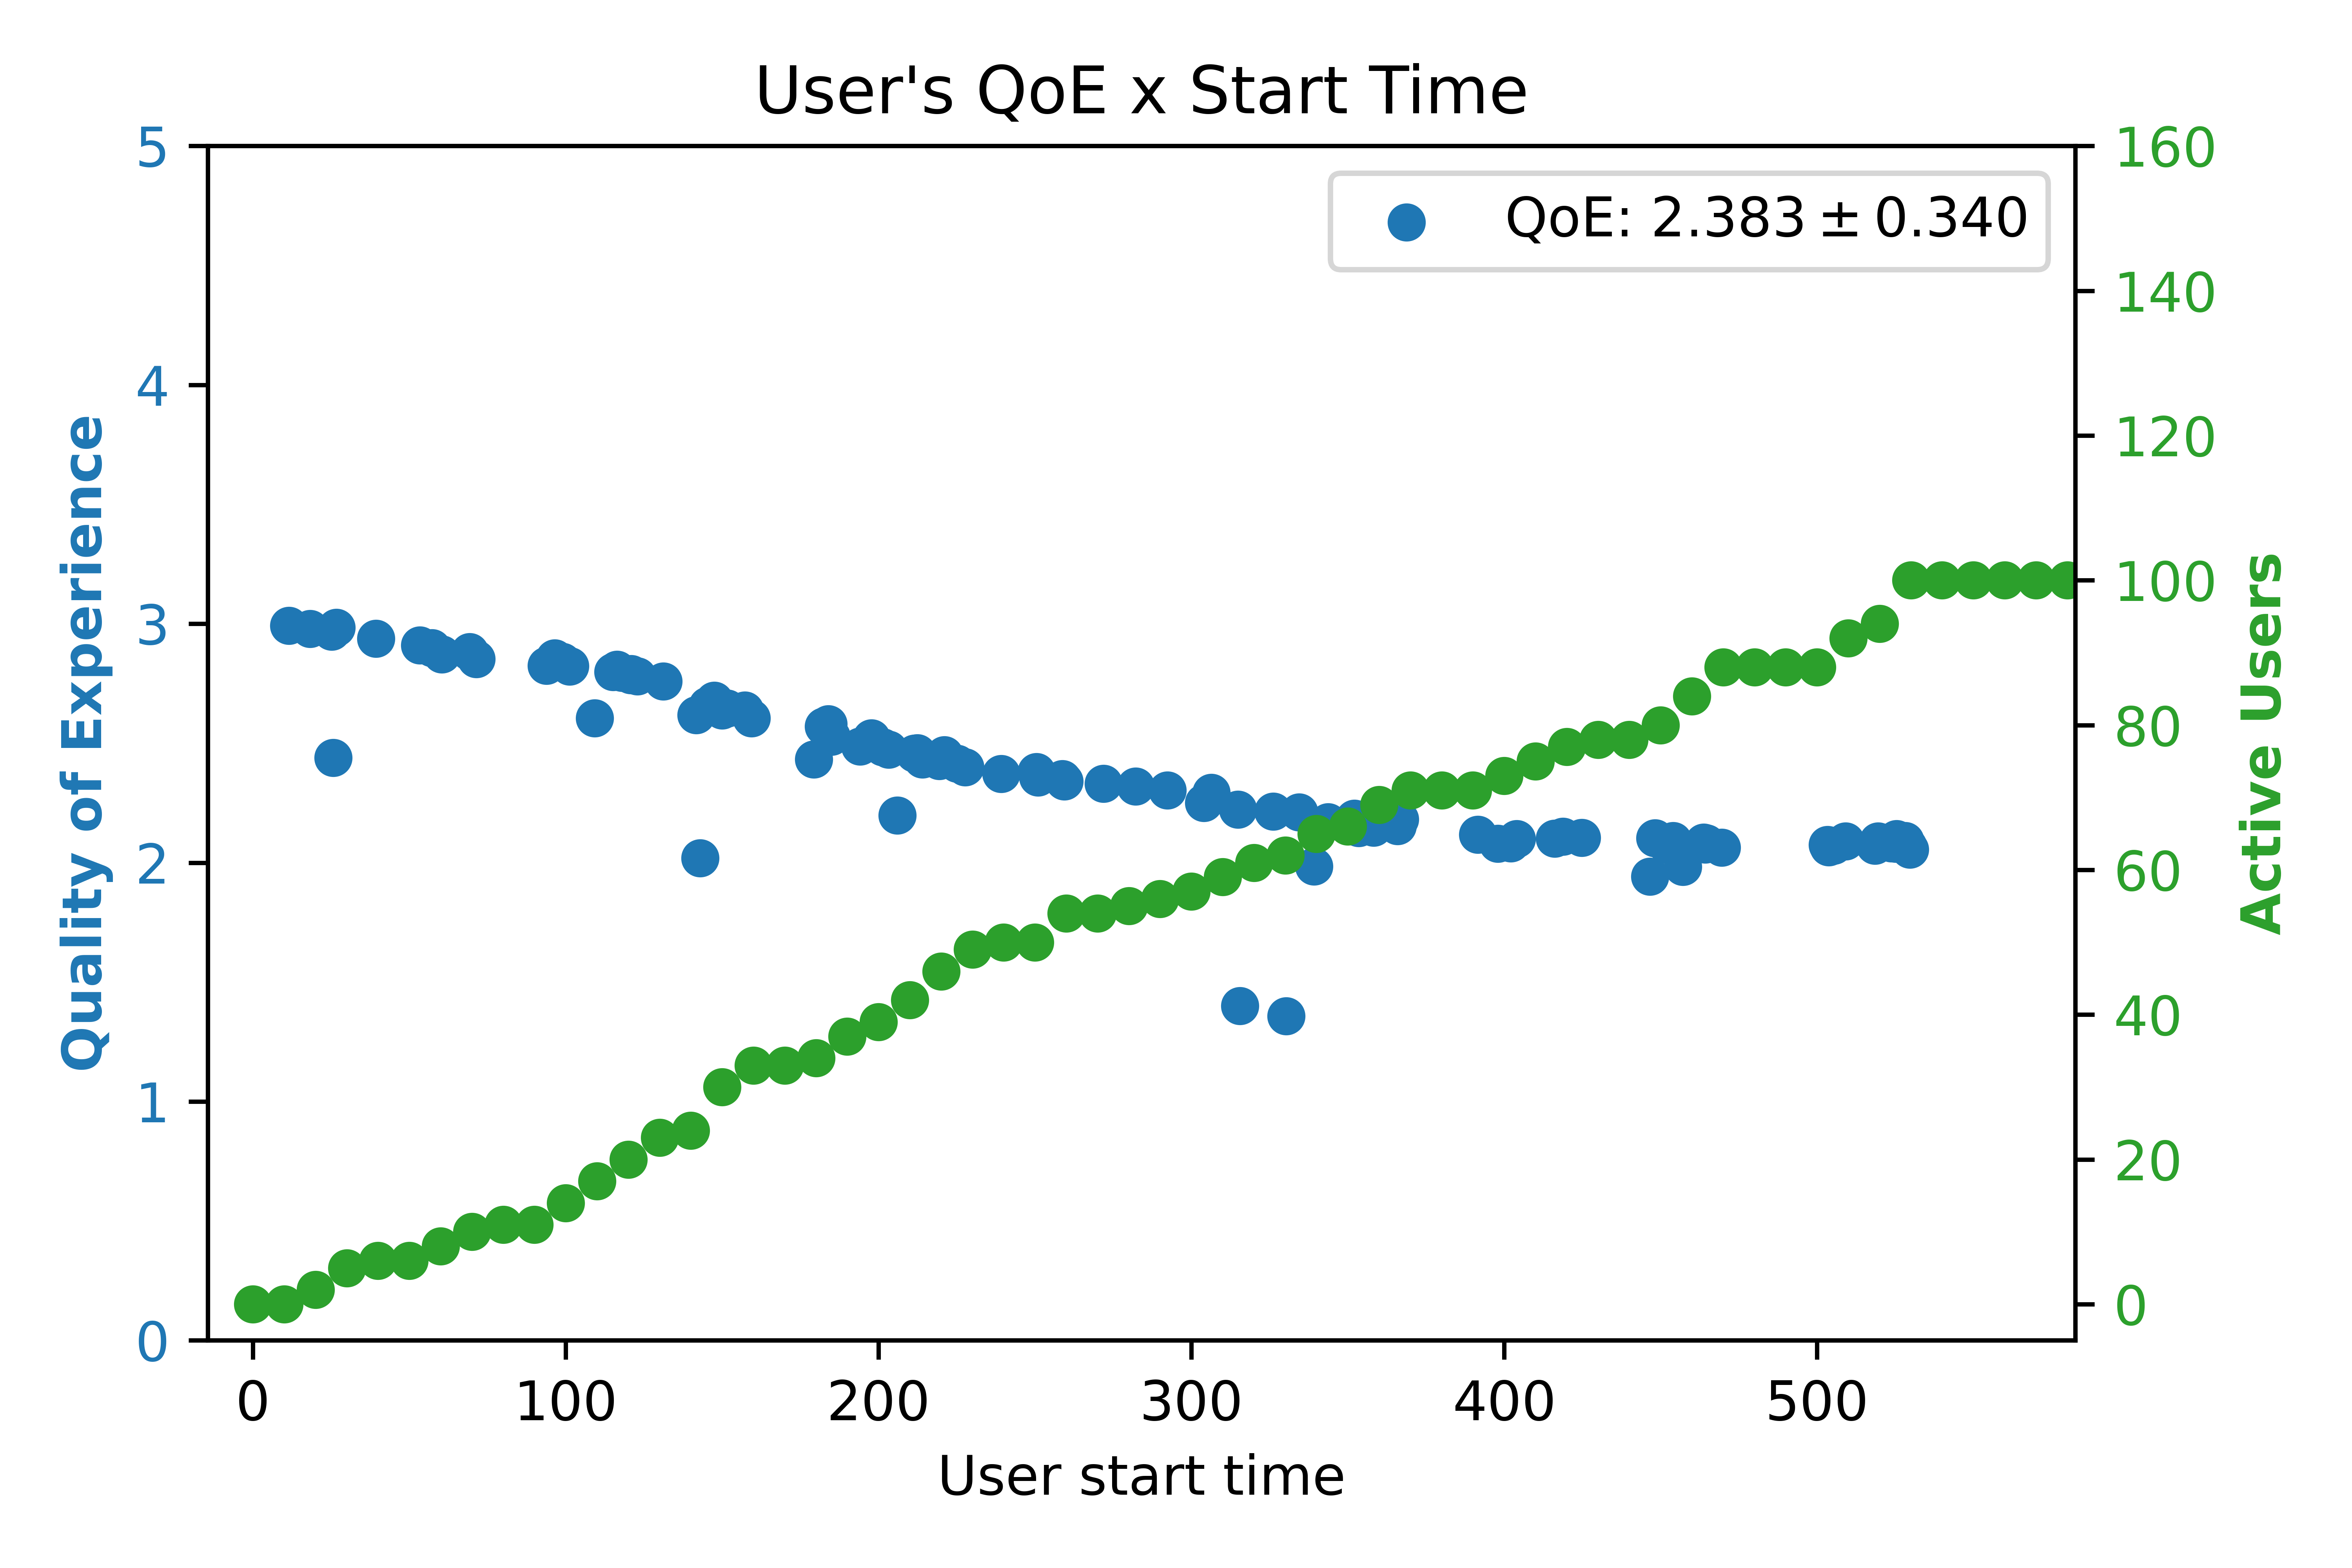
\includegraphics[width=0.31\linewidth]{images/cloud_QoExStartTime25.png}
    \label{fig:plr-comparison-2}
    }
    
    \subfigure[]{
    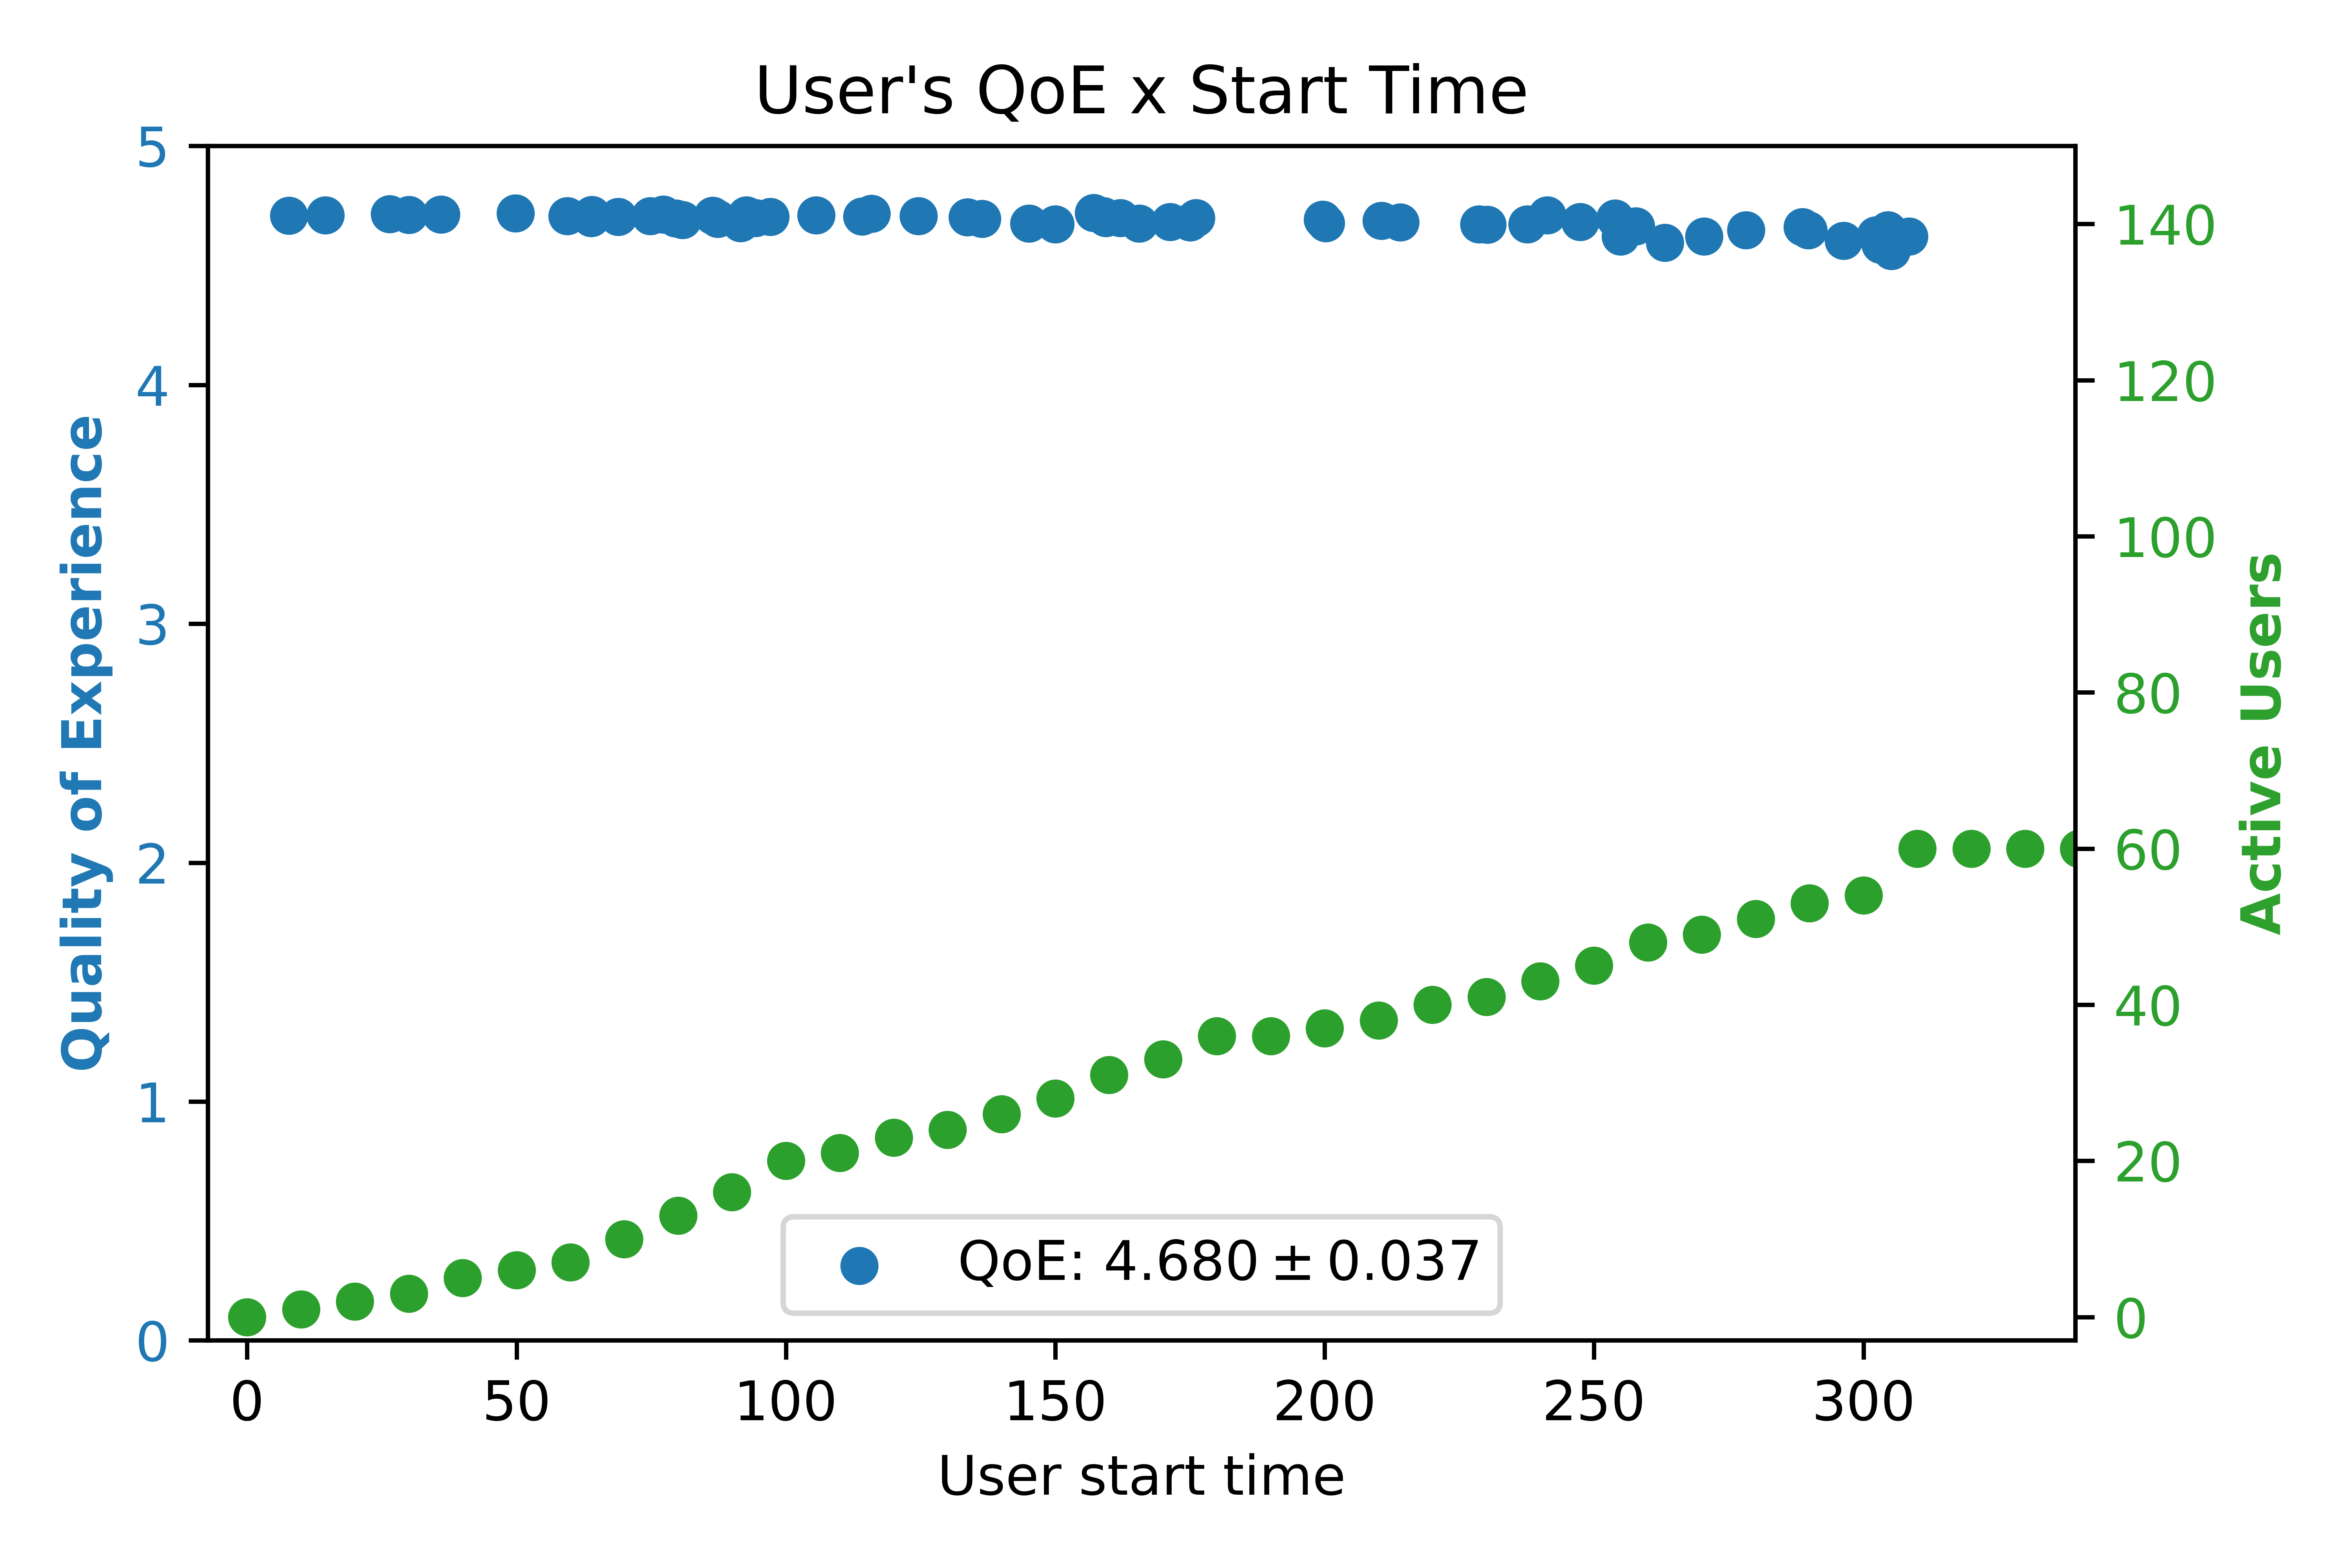
\includegraphics[width=0.31\linewidth]{images/Redicrect_QoExStartTime15.png}
    \label{fig:rssi-comparison-2}
    }
    \subfigure[]{
    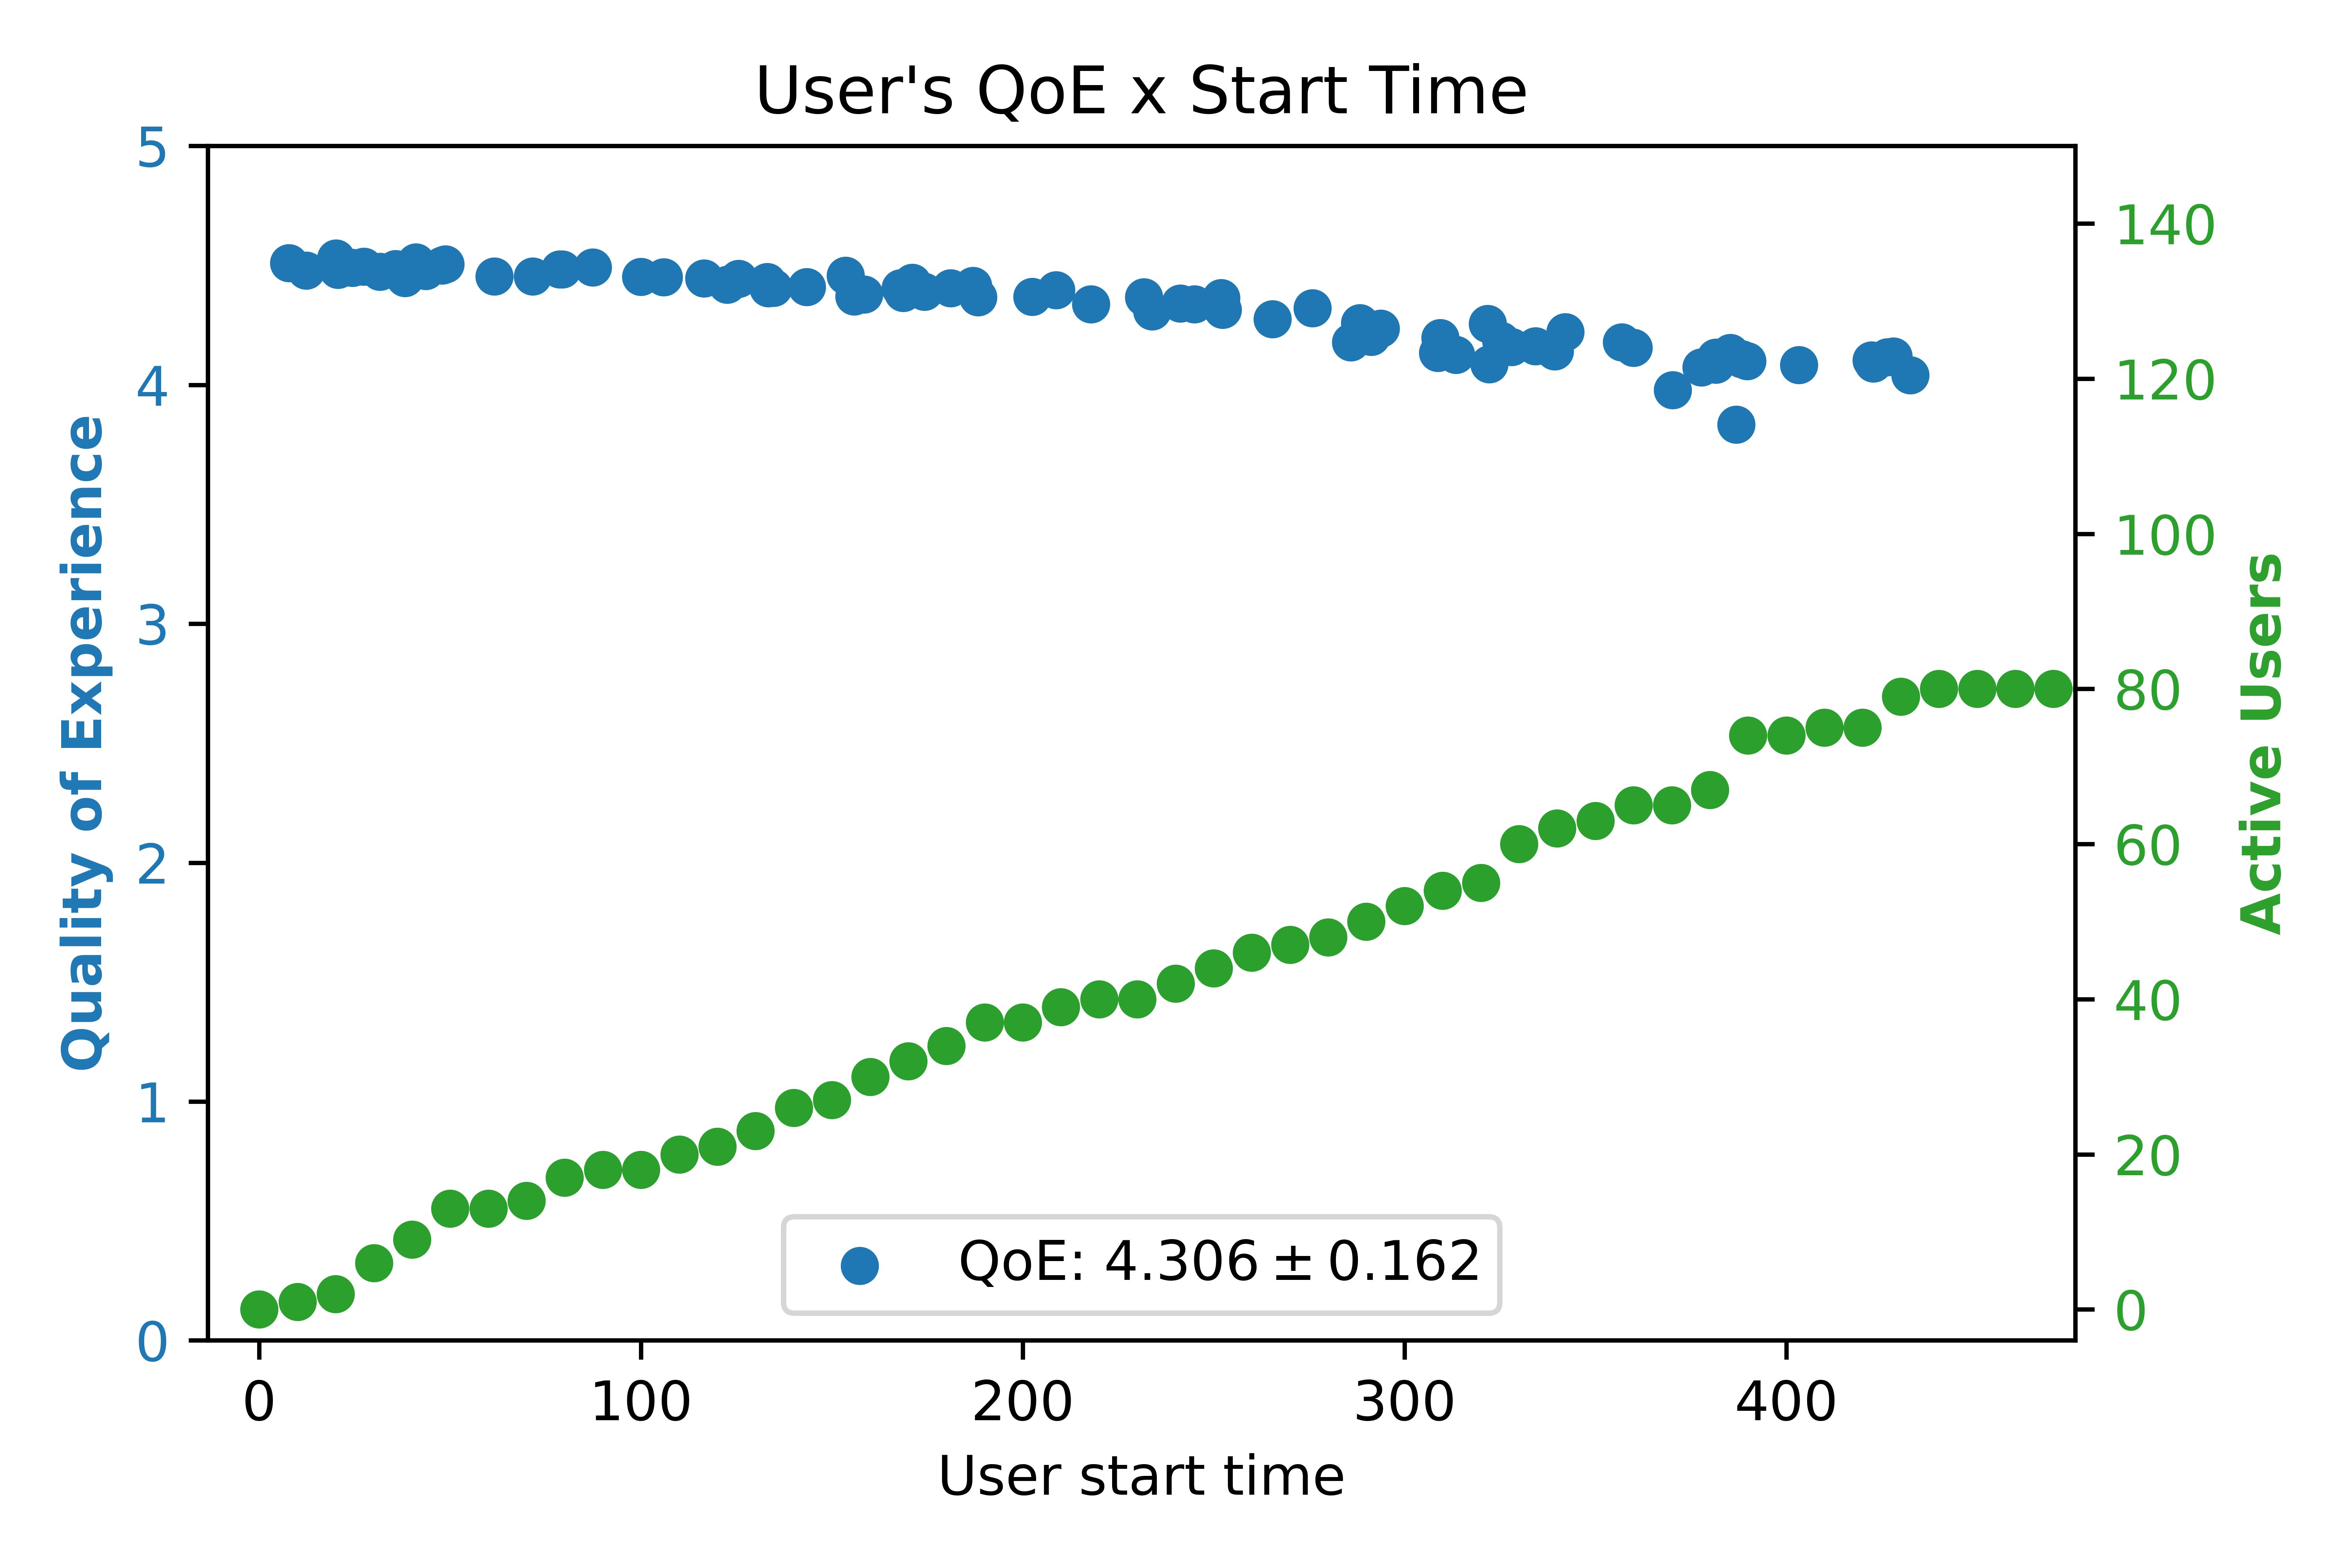
\includegraphics[width=0.31\linewidth]{images/Redicrect_QoExStartTime20.png}
    \label{fig:plr-comparison-2}
    }
    \subfigure[]{
    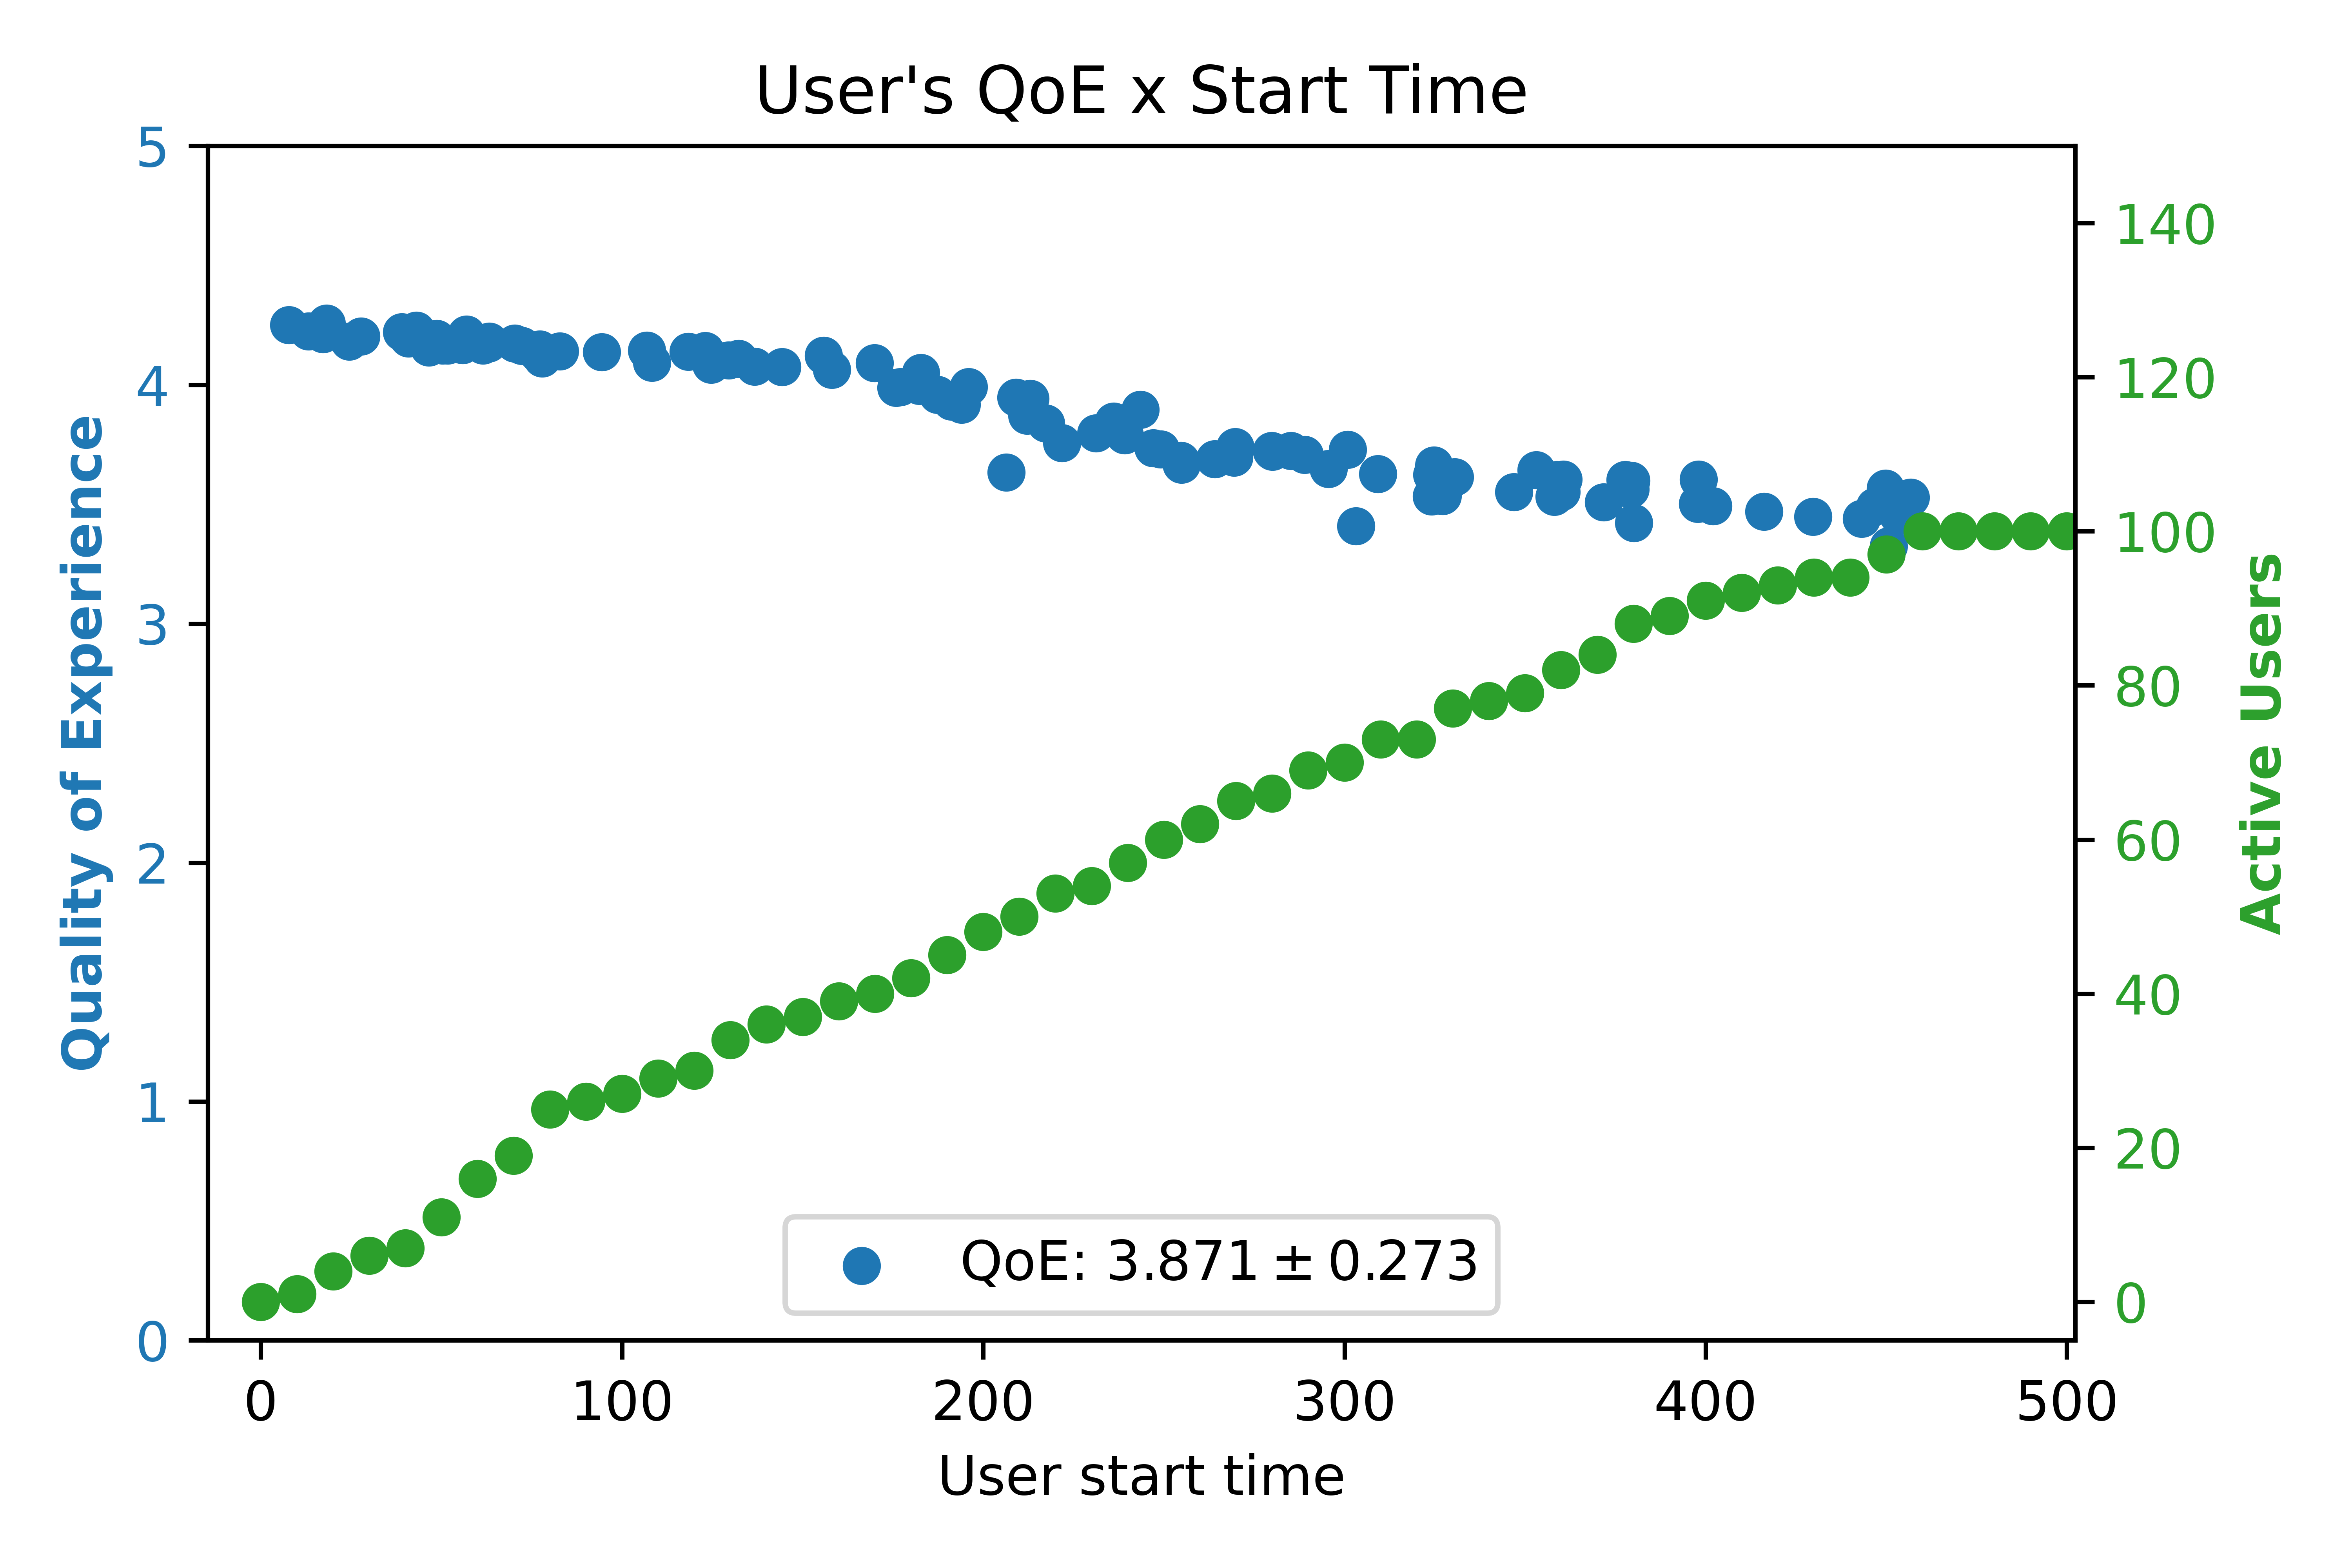
\includegraphics[width=0.31\linewidth]{images/Redicrect_QoExStartTime25.png}
    \label{fig:plr-comparison-2}
    }
    
    \caption{Impact of system on the network performance. Distance \textit{d} between sensor node and antennas of 8m in a semi-NLOS scenario.}
    \label{fig:comparison-qoe-2}
\end{figure*}

\subsection{Results and Discussion}

%As mentioned earlier, the behavior of ABR schemes introduces the problem of selfish decisions when choosing the next segment to be requested. Obviously, different metrics of segment choices lead to different results in the status of buffer occupation and quality of the user's video, which results in a different QoE factor according to the heuristic used.

The experiments illustrated in Figures~\ref{fig:exp-boxplot-15}, \ref{fig:exp-boxplot-20}, and \ref{fig:exp-boxplot-25} show the average QoE calculated by Equation~\ref{eq:qoe-equation} when there are 15, 20, and 25 users per access point requesting videos in the simulated infrastructure. Each boxplot represents the Cloud-only, 1\&2 node and mobility scenarios. The overall average performance of the 1\&2 is better than the Cloud-only and mobility scenarios, mainly due to the choices of nodes at the edge peering nodes for serving the requests from users. 
%
For instance, in the Edge cache experiment, when congestion occurs in intermediate links $e_{0,1}$ e $e_{0,2}$, the edge peering nodes are activated to serve the end-users below those nodes. In this way, the traffic passing through the upward link will now be smoothed out, so the users can have their QoE improved to an excellent level.
%edge peering nodes are activates para atender os usuários abaixo desses nós. Desta forma, os trafego que estava passando pelos link acima agora vão ser suavizados, assim os usuários conseguem melhorar seu QoE resultante para um nível excelente. 
%
Since the users request segments from the closer nodes and with no congestion link in scenarios with Edge cache, as expected, we observe a QoE increase. %Remember that the scenario 1\&2, there is a link congestion monitoring, so when a congestion link is detected, the cache node above the link is activated, and the users are redirected to request the video from the cache node.
%
The performance difference of the Cloud-only and mobility is near one level of satisfaction for 15 and 20 users and approximately two three satisfaction levels with 25 users.


\begin{figure}[!htb]
    \centering
    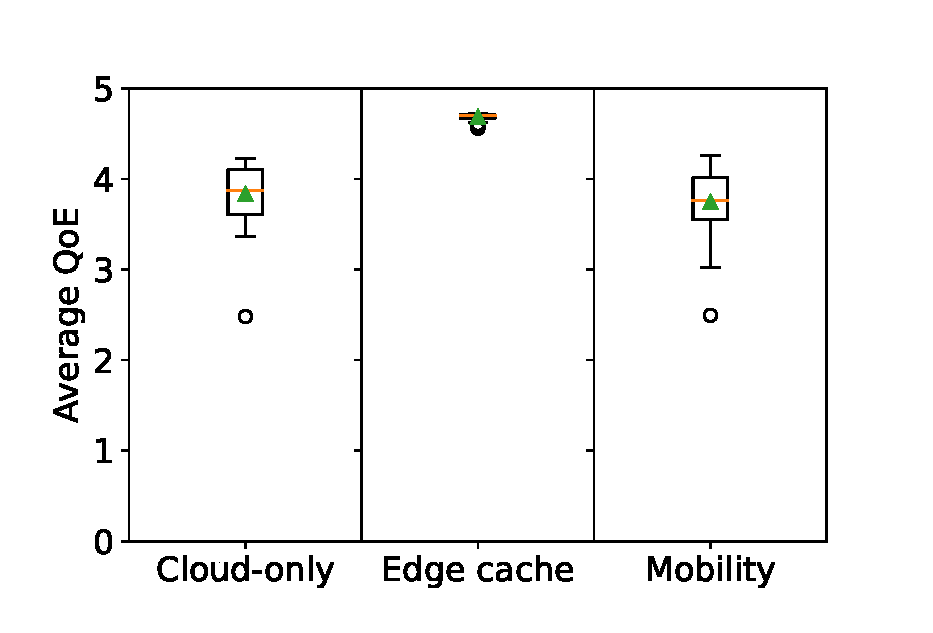
\includegraphics[width=\linewidth]{images/QoEBoxplot-15u-2.eps}
    \vspace{-0.6cm}
    \caption{Average QoE results (15 users per AP).}
    \label{fig:exp-boxplot-15}
\end{figure}

\begin{figure}[!htb]
    \centering
    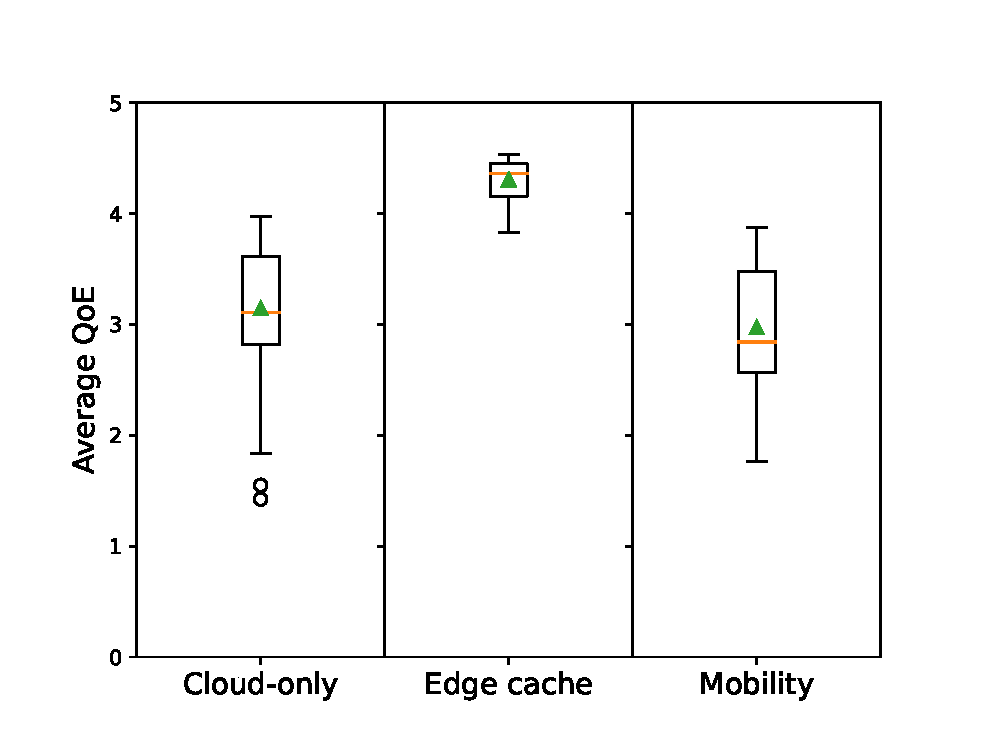
\includegraphics[width=\linewidth]{images/QoEBoxplot-20u-2.eps}
    \vspace{-0.6cm}
    \caption{Average QoE results (20 users per AP).}
    \label{fig:exp-boxplot-20}
\end{figure}

\begin{figure}[!htb]
    \centering
    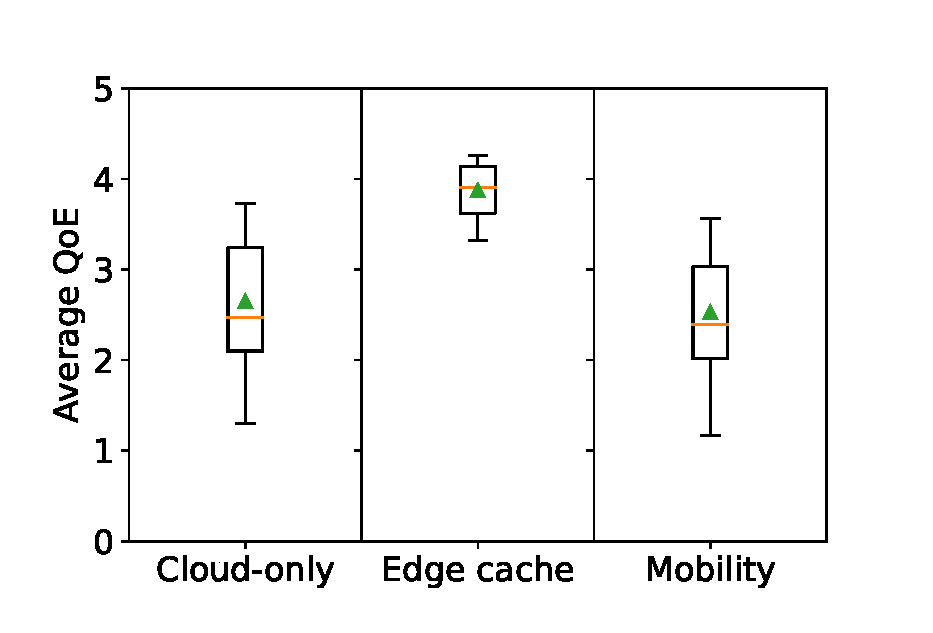
\includegraphics[width=\linewidth]{images/QoEBoxplot-25u-2.eps}
    \vspace{-0.6cm}
    \caption{Average QoE results (25 users per AP).}
    \label{fig:exp-boxplot-25}
\end{figure}


It is important to note that the QoE results of scenarios after mobility are similar to the results of Cloud-only, even with the edge peering nodes using the QoE. This is due to the lack of a rerouting mechanism in real-time when users switch to another AP. The connections between the edge-peering nodes and the users remain unchanged so that the paths through which the packets pass are longer, negatively impacting the performance of the network as a whole.
%Another point to be noted is the average bit rate between different levels. In the scenario with 20 users, level 3 was able to achieve what is necessary to obtain the highest bit rate representation. Thus, network operators can seek to deploy caches during peak hours to provide the best user experience.

Figures~\ref{fig:exp-setup-15}, \ref{fig:exp-setup-20}, and \ref{fig:exp-setup-25} show the final QoE of each user per start time~(time to start the segment requests). Here, we can see the final QoE degradation for each user's entrance during the simulation execution. The red plot represents the number of active users simultaneously. 
As users reach the final QoE in this experiment, it tends to be slightly lower than the previous one. When looking at the final QoE delta between users $u_{i}$ and $u_{i + 1}$, this seems to be irrelevant, but as we increase the delta, the QoE starts to become considerably different. We can also confirm this behavior by showing that as the number of users increases, the average QoE decreases, and the variation between users increases. Also, note that in the simulation with 25 users per AP, the system already shows a degradation in the quality, negatively perceived by the end-user.

\begin{figure}[!htb]
    \centering
    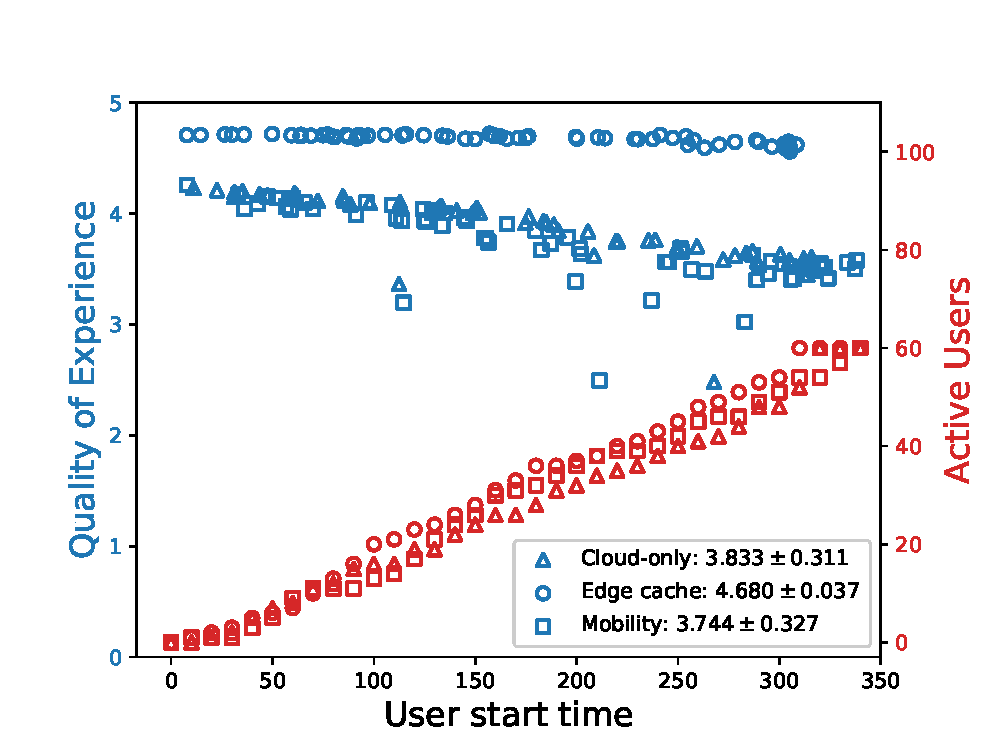
\includegraphics[width=\linewidth]{images/UserQoExUserStartTime15users-2.eps}
    \vspace{-0.4cm}
    \caption{Average QoE for each user (15 users per AP).}
    \label{fig:exp-setup-15}
\end{figure}

\begin{figure}[!htb]
    \centering
    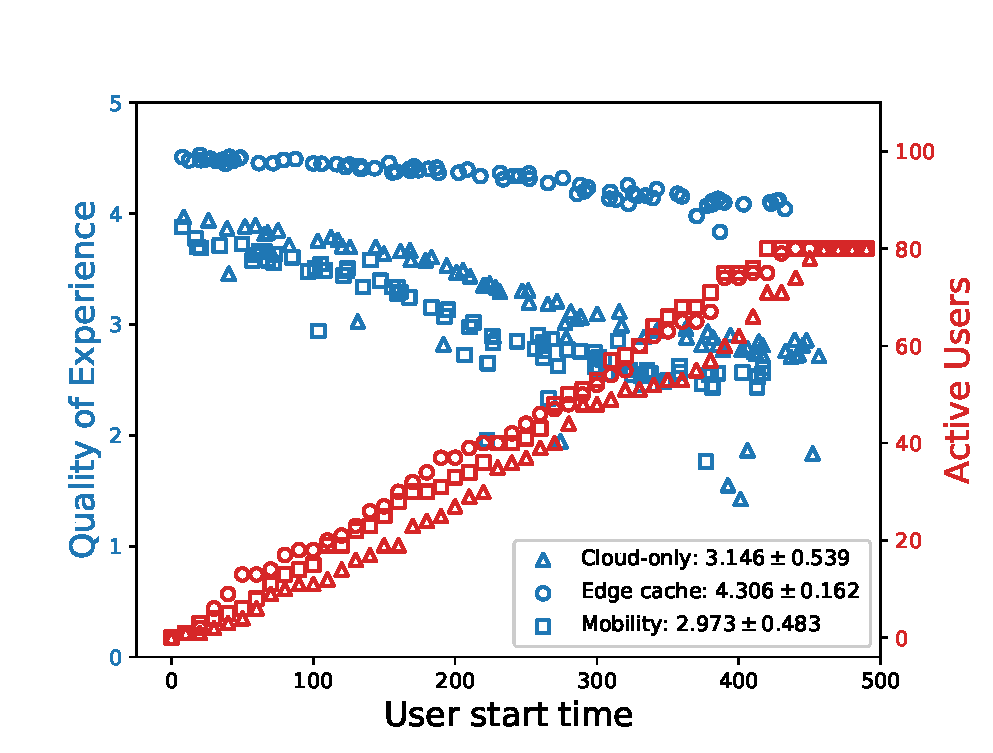
\includegraphics[width=\linewidth]{images/UserQoExUserStartTime20users-2.eps}
    \vspace{-0.4cm}
    \caption{Average QoE for each user (20 users per AP).}
    \label{fig:exp-setup-20}
\end{figure}

\begin{figure}[!htb]
    \centering
    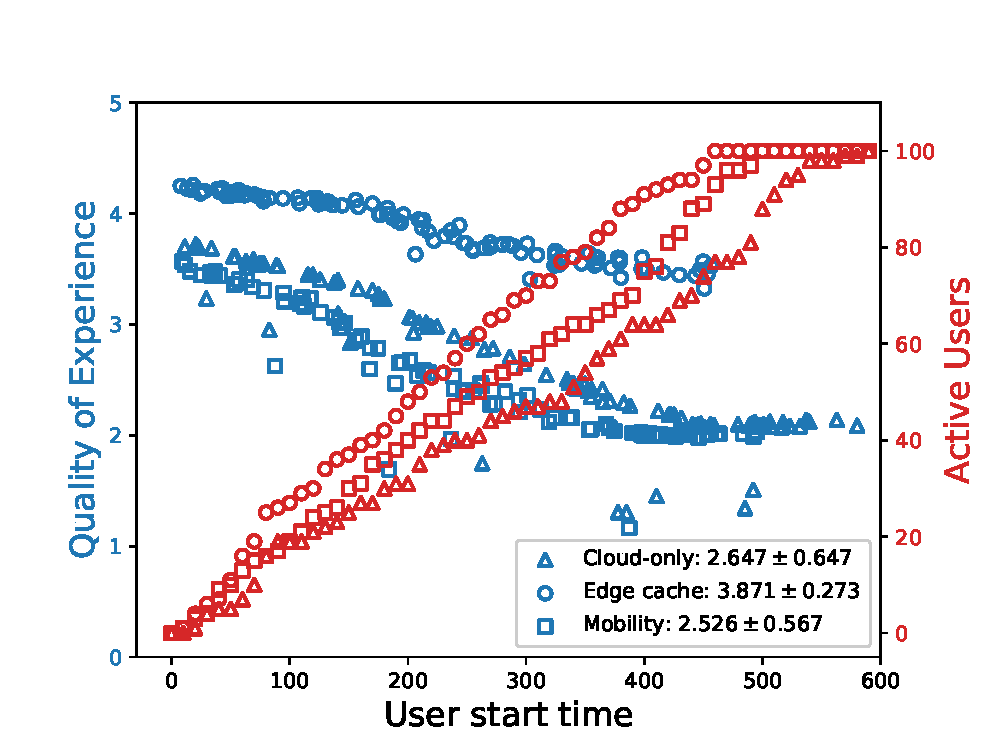
\includegraphics[width=\linewidth]{images/UserQoExUserStartTime25users-2.eps}
    \vspace{-0.4	cm}
    \caption{Average QoE for each user (25 users per AP).}
    \label{fig:exp-setup-25}
\end{figure}

Based on these observations,
a simple strategy of moving the video to the edge can significantly improve the user's QoE. In this way, the video transmission system can provide user satisfaction qualities and keep them watching the video up to the end. However, if there is no correct management of connections in real-time and a dynamic mechanism to tackle with a varying load coming, for example, from the mobility of users, we can conclude that the impact introduced by the AP changes can significantly decrease their QoE. The user experience can end up getting worse even using the edge of the network. Proper management of multimedia content can be done in which the VoD focuses on providing a better QoE for the users' connection changes. A content migration mechanism at the edge and upper tiers can mitigate the problem. Also, performing a rerouting between the active users' connections and the server nodes may help in improving and balance user's QoE.

%Based on these observations,
%a simple strategy of moving the video to the edge can significantly improve the user's QoE. In this way, the video transmission system is able to provide user satisfaction qualities as well as they tend to keep them watching the video until the end. 
%Contudo, caso não ocorra um correcto management das conexões em tempo real,  we can conclude that the impact introduced by the AP changes can decrease significantly the QoE for mobile users. A experiencia do usuário pode acabar se tornando pior mesmo usando a borda da rede. Um gerenciamento adequado do conteúdo multimidia pode ser feito de modo que uma simples migração do conteúdo dentro da borda pode solucionar o problema.